\section{Introduction}\label{introduction}

This chapter describes the models, study sites, and methodologies used in this thesis to address the research questions. The first sections are related to the radiative transfer models and the parameterisation schemes of vegetation canopy heterogeneity that are used in Chapter 4. The next sections describe the photosynthesis model in JULES and briefly summarises the model setups for the experiments performed with the land surface model along the thesis; it also described the flux tower sites used in Chapter 5. The final sections of this chapter are used to describe the global experiment setups, data and methodology. 

\section{Radiative transfer models}\label{section:RTMs}

For most natural woody vegetation such as conifers and savannahs, the spatial distribution of individual tree crowns creates clear spaces where beam radiation propagates without interference of vegetation elements, and because of that the two-stream scheme results in large deviations from the actual amounts of absorbed and reflected radiation \citep{Ni-Meister2010,Kobayashi2012,loew2014}.

For detailed computation of radiation fields within heterogeneous vegetation canopies, radiative transfer schemes can use different complexities to approach the problem. The two-stream scheme was adapted by \citet{Dai2004} to account for sunflecks penetration in order to better simulate the impacts of clearings on fAPAR. Other more complex approaches can be used such as treating vegetation canopies heterogeneously between tree crowns, e.g., in MAESTRA/MAESPA \citep{Wang1990,Duursma2012}, or through a geometrical optical approach, which treat mixtures of individual trees and multiple scattering with foliage clumped within tree crowns, e.g., in the GORT model \citep{Li1995}. However, these 3D models cannot be directly used in LSMs due to their extreme computational power demand \citep{Yang2001} and the high number of required vegetation structural parameters \citep{loew2014}.

%\subsection{The two-stream scheme with vegetation clumping: parameterisation schemes}\label{section:parameterisations}
\subsection{The two-stream scheme in JULES} 

The two-stream version used in this thesis was extracted from the JULES model. The JULES model is the UK community land surface model designed to be interfaced with the UK Met Office Unified Model \citep{Walters2014} by predicting fluxes of heat, water, and carbon between the land surface and the atmosphere. It originates from the Met Office Surface Exchange Scheme (MOSES) \citep{Cox1999}, and it includes the TRIFFID (Top-down Representation of Interactive Foliage and Flora Including Dynamics) dynamic vegetation model \citep{Cox2001}. The physical basis of JULES is common to most of the land surface models and are described in details in \citet{Best2011} and \citet{Clark2011}. 

JULES uses a default number of 10 layers with equally distributed LAI to calculate the radiative transfer in the canopy following the two-stream scheme. The extinction properties of leaves are prescribed by PFTs and are given by leaf reflectance ($\rho_{leaf}$) and transmittance ($\tau_{leaf}$) in the PAR and NIR wavebands, and canopy leaf angle distribution can be either spherical, or horizontal, but along this thesis the spherical approximation was used, where G-funtion = 0.5. The amount of absorbed incident radiation at each layer is therefore determined by Sun zenith angle, incident direct and diffuse radiation at the top of the canopy, and the extinction coefficients.

A further improvement to the estimation of absorbed radiation within the canopy considers penetration of sunflecks (can\textunderscore rad\textunderscore mod = 5), which excludes the scattering component and therefore corresponds to the direct component of the direct beam radiation \citep{Clark2011}. The term associated with sunflecks is not included in the original formulation of the two-stream scheme. Following \citet{Dai2004} as implemented in \citet{Mercado2009}, radiation fluxes are separte into direct beam radiation, scattered direct beam, and diffuse radiation, and it is assumed that sunlit leaves absorb all types of radiation while shaded leaves absorb only diffuse radiation. The fraction of sunlit leaves (f$_{sun}$), is defined as:
\begin{equation}
 f_{sun} = e^{\frac{G(\mu)}{\mu} \cdot LAI}
\end{equation}\label{eq:fsun}
\noindent where G($\mu$) is the G-function \citep{Ross1981}, $\mu$ is the cosine of Sun zenith angle, and LAI is the total leaf area index. For each canopy layer \textit{i} with leaf area increment dL$_c$, the fraction of sunlit leaves, fraction of absorbed direct beam radiation, fraction of scattered direct beam, and fraction of absorbed diffuse radiation are described in \citep{Clark2011}. The fractions of the incident radiation above the canopy which are absorbed by sunlit leaves and shaded leaves separately in each leaf area increment within the canopy are dependent on the amount of incident diffuse shortwave radiation.

%Several previous studies have suggested with observations and detailed modelling approaches that vegetation 3D structure influences radiation partitioning and other land surface related processes \citep{Nilson1971,Wang1990,Chen1996,Kucharik1999,Yang2001,yang2003,Jonckheere2004,pinty2006,Chen2008,Ni-Meister2010,Widlowski2011,Kobayashi2012,Loew2014}.

%For most natural woody vegetation such as conifers and savannahs, the spatial distribution of individual tree crowns creates clear spaces where beam radiation propagates without interference of vegetation elements, and because of that the two-stream scheme results in large deviations from the actual amounts of absorbed and reflected radiation \citep{Ni-Meister2010,Kobayashi2012,Loew2014}.

%For detailed computation of 3D radiation fields within complex vegetation canopies, radiative transfer schemes can use a geometrical optical approach and treat mixtures of individual trees and multiple scattering with foliage clumped within tree crowns, e.g., in the GORT model \citep{Li1995}. Another approach is to treat it heterogeneously between tree crowns, e.g., in MAESTRA/MAESPA \citep{Wang1990,Duursma2012}, among others more complex approaches. However, these models cannot be directly used in GCMs due to their extreme computational power demand \citep{Yang2001} and the high number of required vegetation structural parameters \citep{Loew2014}. 

%The two-stream scheme is still preferably used because of its simplicity, speed, and suitability to run over large areas, the use of effective radiative state variables to express the properties of 3D vegetation canopy systems makes a simpler model to analogously simulate the radiation balance of more complex 3D models \citep{Pinty2004,pinty2006}, hereafter clumping indices.

%Thus the clumping indices account for all phyto and woody elements composing the vegetation canopy, and when its value is greater than 1, it is an indication of specific structural canopy conditions associated with significant amounts of woody elements \citep{pinty2006}. 

%The first clumping index was proposed by \citet{Nilson1971} and it is associated with the heterogeneous nature of the canopy volume \citep{Norman1974,chen1992,Chen1996}, often used at the tree resolution, and revisited later on by other authors \citep{Pinty2004,pinty2006}, who used the same scientific proposition to account for structural heterogeneity of different radiative media at stand scale as whole, which is usuful for direct comparison with eddy covariance data and associated use with satellite products.

%Few other authors \citep{Kucharik1999,pinty2006,Ni-Meister2010} attempted to formulate simplified modelling approaches to resolve vegetation clumping at several levels of organisation, in order to address the major differences in shortwave radiation partitioning between 1D and 3D radiative transfer schemes over non-homogeneous forest canopies.

%The next sections will describe four different clumping indices to address vegetation heterogeneity in the modified two-stream scheme. Evaluations will be performed against a benchmarking exercise of radiation transfer in vegetation canopies, the RAMI4PILPS experiment \citep{Widlowski2011}.

\subsection{Tree-based model: MAESPA}\label{section:maespa}
The MAESTRA/MAESPA model \citep{Wang1990,Medlyn2004,Medlyn2007,Duursma2012} represents a forest canopy as an array of tree crowns, whose positions and dimensions are specified. The radiation routines are described in detail by \citet{Wang1990}. The canopy consists of individual tree crowns, which are described by a basic shape (one of several shapes, including ellipsoids, cylinders and cones), length, height to crown base, and width (in x and y directions). Radiation calculations are performed only for a set of target crowns specified by the user. The distribution of leaf area within the target crown is specified, as is the leaf angle distribution. The target crown is divided into usually 60 grid points, and the radiation penetrating to each grid point is calculated for three wavebands (PAR, NIR and thermal infra-red, TIR) based on shading within the crown, shading by neighbouring trees, the location of the sun, and whether radiation is direct or diffuse. Direct, diffuse and scattered radiation are considered separately. Scattering of radiation is approximated following \citet{Norman1979}. Leaf area within crowns is assumed to be distributed randomly \citep{Wang1990}. At each grid point, leaf area is separated into sunlit and shaded leaf area (Norman, 1993). The model has previously been applied to study canopy carbon and water fluxes of \textit{Picea sitchensis} \citep{Wang1990}, \textit{Pinus radiata} \citep{McMurtrie1993}, \textit{Betula pendula} \citep{Wang1998}, and \textit{Pinus taeda} \citep{Luo2001}. 
%Using the $R$ (R Development Core Team, 2011) package, Maeswrap (Duursma, 2015), the 3D stand scenes were graphically reproduced in 3D.

\subsection{Geometric optics model: GORT}\label{section:gort}
The GORT model was developed to describe the effects of three-dimensional canopy structure on the radiation environment and to characterise the heterogeneous radiation environment in natural vegetation at the forest stand scale \citep{Ni-Meister2010}. Merging theory from geometric optics and radiative transfer, the GORT model treats vegetation canopies as assemblages of randomly distributed tree crowns of ellipsoidal shape. The tree crowns are filled with leaves that absorb and scatter radiation passing through the crown. Principles of radiative transfer are used in describing the multiple scattering of leaves inside crowns and the multiple scattering among crowns and the ground surface. The GORT model was extended by \citet{Ni1997} to include the vertical canopy gap probability profile. For this exercise the PAR radiation spectrum was centred in 550 nm, and NIR in 850 nm.

\subsection{Monte Carlo ray-tracing model: raytran}\label{section:raytran}

%The RAMI4PILPS \citep{Widlowski2011} suite of experiments was designed to evaluate the accuracy and consistency of shortwave radiative transfer formulations as used in LSMs by evaluating different RT models against the extensively verified 3D reference Monte Carlo ray-tracing model, known as raytran \citep{Govaerts1995}.

%One of the specificities of the RAMI4PILPS suite ofexperiments is that model simulations can be compared against a reference data set of relatively well known uncertainty. The latter was provided by the 3D Monte Carlo ray‐tracing model known as raytran \citep{Govaerts, 1998}. 

The raytran model has been compared extensively against goniometer measurements \citep{Govaerts1995}, field observations \citep{Widlowski2005}, and more systematically, against other RT models in the context of the RAMI activity \citep{Pinty2001,Pinty2004,Widlowski2007}. Due to its excellent performance with respect to energy conservation, and its matching of analytical solutions to within 10$^{−4}$ on average, the raytran model was identified as one of six credible 3D canopy RT models and chosen to contribute to the development of a reference dataset against which other radiative transfer models could then be evaluated. This reference data set is based on the RAMI simulations of all six credible 3D Monte Carlo models (having a mutual divergence of less than 1\% over many thousands of model runs) and has become the cornerstone of the RAMI On‐line Model Checker \url{http://romc.jrc.ec.europa.eu/} a web based facility for the autonomous benchmarking of canopy reflectance models \citep{Widlowski2008}.

The ray-tracing code used in the RAMI4PILPS experiment allows the explicit representation of radiation transfer in arbitrarily complex scenes \citep{Govaerts1998} by implementing a Monte Carlo approach where the fate of millions of individual rays are followed as they travel through the computer simulated scene. This model implements the most detailed and most faithful simulations of radiation transfer, but as other complex models is rather expensive computationally.

\section{Vegetation canopy architecture parameterisation schemes}

%Several previous studies have suggested with observations and detailed modelling approaches that vegetation 3D structure influences radiation partitioning and other land surface related processes \citep{Nilson1971,Wang1990,Chen1996,Kucharik1999,Yang2001,yang2003,Jonckheere2004,pinty2006,Chen2008,Ni-Meister2010,Widlowski2011,Kobayashi2012,Loew2014}.

%For most natural woody vegetation such as conifers and savannahs, the spatial distribution of individual tree crowns creates clear spaces where beam radiation propagates without interference of vegetation elements, and because of that the two-stream scheme results in large deviations from the actual amounts of absorbed and reflected radiation \citep{Ni-Meister2010,Kobayashi2012,Loew2014}.

%For detailed computation of 3D radiation fields within complex vegetation canopies, radiative transfer schemes can use a geometrical optical approach and treat mixtures of individual trees and multiple scattering with foliage clumped within tree crowns, e.g., in the GORT model \citep{Li1995}. Another approach is to treat it heterogeneously between tree crowns, e.g., in MAESTRA/MAESPA \citep{Wang1990,Duursma2012}, among others more complex approaches. However, these models cannot be directly used in GCMs due to their extreme computational power demand \citep{Yang2001} and the high number of required vegetation structural parameters \citep{Loew2014}. 

The two-stream scheme is still preferably used in LSMs because of its simplicity, speed, and suitability to run over large areas. Effective radiative state variables, hereafter clumping indices, are often used to express the properties of 3D vegetation canopy systems and makes a simpler model to analogously simulate the radiation balance of more complex 3D models \citep{Pinty2004,pinty2006}.

Thus the clumping indices account for all phyto and woody elements composing the vegetation canopy, and when its value is greater than 1, it is an indication of specific structural canopy conditions associated with significant amounts of woody elements \citep{pinty2006}. 

The first clumping index was proposed by \citet{Nilson1971} and it is associated with the heterogeneous nature of the canopy volume \citep{Norman1974,chen1992,Chen1996}, often used at the tree resolution, and revisited later on by other authors \citep{Pinty2004,pinty2006}, who used the same scientific proposition to account for structural heterogeneity of different radiative media at stand scale as whole, which is usuful for direct comparison with eddy covariance data and associated use with satellite products.

Few other authors \citep{Kucharik1999,pinty2006,Ni-Meister2010} attempted to formulate simplified modelling approaches to resolve vegetation clumping at several levels of organisation, in order to address the major differences in shortwave radiation partitioning between 1D and 3D radiative transfer schemes over non-homogeneous forest canopies.

%The next sections will describe four different clumping indices to address vegetation heterogeneity in the modified two-stream scheme. Evaluations will be performed against a benchmarking exercise of radiation transfer in vegetation canopies, the RAMI4PILPS experiment \citep{Widlowski2011}.

\subsection{The clumping index of Nilson (1971)}

To consider the non-random spatial distribution of leaves, \citet{Nilson1971} first proposed a Markov-chain model introducing an additional quantity, $\Omega$, into Eq.~\ref{equation:pgapnilson}:
\begin{equation}
P_{gap}(\theta) = \exp{(\frac{-G(\theta)  LAI  \Omega}{cos(\theta)})}
\label{equation:pgapnilson}
\end{equation}
\noindent where P$_{gap}$($\theta$) is the direct transmissivity, G($\theta$) is the G-function \citep{Ross1981}, LAI is the total scene LAI, $\theta$ is the Sun zenith angle, $\Omega$ is the clumping index.

%The complete zenith profile of P$_{gap}$($\theta$) was then calculated by the MAESPA model as 1 - fAPAR for a black canopy, i.e., with leaf reflectance and transmittance equal zero, as well as soil albedo. As MAESPA is considered to be a robust tool to calculate absorbed PAR, by appling the Beer\textquotesingle s law to a black body, in this case the different canopy densities described by the RAMI4PILPS scenes, if the light is not absorbed by the vegetation canopy, the light is then transmitted through it. The clumping index was derived as the adjusted angular coefficient of the inverted Eq.~\ref{equation:pgapnilson}, and the values are summarised in Table~\ref{tab:niclumpparameters}.

\subsection{The clumping index by Kucharik et al. (1999)}
The parameterisation described in this subsection was developed by \citet{Kucharik1999}. The authors used measurements of LAI and gap fraction made with MVI (Multiband Vegetation Imager) \citep{Kucharik1997} obtained during the BOREAS (Boreal Ecosystem-Atmosphere Study) \citep{Sellers1997} field campaigns of 1994-1996 to derive a semi-empirical relationship between $\Omega(\theta)$ and solar zenith angle ($\theta$). 

In this method, two key quantities are needed: (i) the fraction of ground area covered by the horizontal projection of crown envelopes ($f_c$) (from nadir view), which is a function of the typical tree crown diameter ($D$), and tree stem spacing ($\lambda$), or stem density, within a study plot; and (ii) an estimate of crown porosity ($\Phi$); this quantity is related to foliage density and defined as the gap fraction within crown envelopes divided by $f_c$.
 
A series of zenith gap fraction measurements were needed along a transect beneath a canopy to partition the total gap fraction ($f_{gap},t(0)$) between within-crown and between-crown gaps, and  an estimate of the total fraction of ground area covered by the horizontal projection of crown envelopes ($f_c$). To obtain $f_c$, the typical crown silhouette area ($\pi R^2$, where $R$ is the crown radius in the horizontal direction) is multiplied by the number of crowns and divided by the total ground unit area on which the stem density is based. If $f_c$ is greater than 1, crowns typically overlap in the forest, and the entire value of $f_{gap},t(0)$ can be defined as within-crown gap fraction ($f_{gap},c(0)$). The total gap fraction occurring between-crowns ($f_{gap},b(0)$) can be estimated by $1 - f_c$, and $f_{gap},c(0)$ is therefore approximated by $f_{gap},t(0) - f_{gap},b(0)$. If the value of $f_{gap},c(0) < 0$, it can be assigned a value of 0 for all practical purposes. 

Crown porosity ($\Phi$) is determined by dividing $f_{gap},c(0)$ by $f_c$ ($\Phi$ = $f_{gap},c(0)/f_c$). The value of $\Phi$ may be described as a normalised within-crown gap fraction. Generally, an error of about 0.05 exists in determining $f_c$ and $\Phi$ by using an average crown radius and tree stem density rather than the actual model calculations of $f_c$. However, the authors indicated that these errors are not of concern when estimating $\Omega(0)$ using the gap-fraction partitioning strategy.

Values of $\Phi$ and $f_c$ were then used to determine a value of $\Omega$(0) that was consistent with calculations resulting from numerical simulations of the canopy gap-size distribution. A non-linear least-squares fit to approximately 250 Monte Carlo simulations (analysing values of $\Omega(0)$) was performed for values of $f_c$ $\geq$ 0.20, and for all simulated values of $\Phi$. A separate fit to the entire set of model data was performed for 0.04 $\geq f_c \geq$ 0.30. For sparse canopies where $f_c < 0.20$, a value of $\Omega(0)$ could still be determined. 

Ten equations were solved simultaneously to determine 10 coefficients ($a_0$, ..., $a_9$) that describe the relationship between values of $\Omega(0)$, $f_c$, and $\Phi$. To characterise the angular dependence of $\Omega(\theta)$, a minimum value of $\Omega(\theta)$ was determined at $\theta$ = 0$^{\circ}$ and a value of $\Omega(\theta)$ was needed at $\theta$ = 90$^{\circ}$. Because it was assumed that $\Omega(\theta)$ reaches its maximum value at $\theta$ = 90$^{\circ}$, \citet{Kucharik1999} refer to this value as the maximum possible element clumping index, $\Omega_{max}$, and defines it as:
\begin{equation}
\Omega_{max} = \Big(\frac{ND}{\sqrt{A}}\Big)^{0.7}
\label{equation:clumpmax}
\end{equation}
\noindent where $N$ is number of stems within ground area $A$, and $D$ is crown diameter. If $ND/\sqrt{A} > 1$, then the value of $\Omega_{max} = 1$. The angular dependence of $\Omega(\theta)$ was defined by \citet{Kucharik1999} following the equation: 
\begin{equation}
\Omega = \Omega(\theta) = \frac{\Omega_{max}}{[1 + b\exp(-k(\theta)^p)]}
\label{equation:clumptheta}
\end{equation}
\noindent where $k$ is constant (usually $k$ = 2.2), $\theta$ is zenith angle expressed in radians, and $b$ is solved from a rearrangement of Eq.~\ref{equation:clumptheta} using a known value of $\Omega(\theta)$ (e.g., $\theta$ = 0$^{\circ}$). A quantitative comparison of results produced using Eq.~\ref{equation:clumptheta} with the best-fit curves suggested that a value for $p$ can be approximated by an equation on the form:
\begin{equation}
p = -0.461\chi + 3.8
\label{equation:pchi}
\end{equation}
\noindent where $\chi$ is the ratio of crown depth to crown diameter. Generally, if $\chi$ is $\leq$ 1.0, $p$ = 3.34. 

\subsection{The structure factor of Pinty et al. (2006)}

The clumping index of \citet{pinty2006} is given by:
\begin{equation}
\Omega = \zeta(\mu) \approx a + b \cdot (1 - \mu)
\label{equation:structurefactor}
\end{equation}
\noindent where $\mu$ is the cosine of $\theta$, $a = \zeta(\mu=1)$ is the parameter corresponding to an overhead Sun, and $b$ the parameter responsible for include the effects of a range of different Sun geometries. In the particular case of an overhead Sun ($\mu$=1), $a$ is also equal to:
 \begin{equation}
\zeta(\mu=1) = -\ln{(1 - F_c)}\frac{2}{LAI}
\label{equation:structurefactora}
\end{equation}
\noindent where $F_c$ is the true vegetation cover (accounting for within and between crown gaps) obtained for a black canopy representation ($\rho_{leaf} = \tau_{leaf} = 0.0$) of the total incident radiation minus direct transmissivity with an overhead Sun (1 - P$_{gap}(\theta = 0^{\circ}$)). Both parameters are used to account for vegetation canopy heterogeneity and modify the radiation path length.

\subsection{The clumping index by Ni-Meister et al. (2010)}
\citet{Ni-Meister2010} developed an analytical expression for clumping based on stem density ($\lambda$), crown radius ($R$) and LAI. In here, only the equation used for spherical crowns is shown, however. The analytical solution for the modified clumping index in Beer\textquotesingle s law is expressed as, 
\begin{equation}
\Omega = \gamma = \frac{3}{4\tau_0R}\Big(1 - \frac{1 - (2\tau_0R + 1)\exp(-2\tau_0R)}{2\tau_0^2R^2}\Big)
\label{equation:clumpNi}
\end{equation}
\noindent where $\tau_0r = 3 G LAI/ 4 \lambda \pi \cdot R^2$ for spherical crowns. 

The authors validated the analytical solutions for clumping factor with the ones calculated by the full GORT model \citep{Li1995}, which was specifically developed to describe the effects of 3D canopy structure on the radiative balance and to characterise the heterogeneous radiative balance in natural vegetation at the forest stand scale.

\section{Handling vegetation heterogeneity in current LSMs}\label{sec:fveg}

%Full 3D radiative transfer models require a large number of parameters, and a high computational demand, thus, 1D radiative transfer approaches are still preferably used \citep{yang2003,loew2014}. However,
More simplified approaches to handle sparse vegetated canopies have been implemented in LSMs and are widely used \citep{loew2014}. The vegetation cover approach divides one grid cell in a number of tiles, where each tile has its own characteristics. The possible number of tiles and their parameters depend on each LSMs.

Suppose a model grid cell with area $A$, which is assumed to be fully covered (100\%) by a particular vegetation type. In the case of sparser canopies, e.g. savannahs, the area $A$ is covered by a dominant vegetation type, usually taller trees, but often presents a second vegetation type, for example, understory vegetation (e.g. shrubs, grass) and so on, or part of the grid with no vegetation at all is covered by bare soil. The total area $A$ is thus defined as,
\begin{equation}
A = f_{veg} + f_{under}
\label{equation:area}
\end{equation}
\noindent where $f_{veg}$ is the fractional coverage of the major vegetation type and $f_{under}$ can correspond to a different vegetation type or the soil surface.
In this case $f_{under}$ is equivalent to the between-crown gaps. The total direct transmissivity, or the gap probability with Sun above head ($\theta$ = 0$^{\circ}$) is always greater than or equals to $f_{under}$. Figure~\ref{f:loew2014} from \citet{loew2014} shows a representation of a sparse vegetation canopy with $f_{veg}$ being the percentage of the area covered by a single vegetation type, $f_{under}$ is the remaining area, and P$_{gap}$($\theta$=0$^{\circ}$) as being $f_{under}$ plus the within-crown gap probability.

\begin{figure}
\centering
\includegraphics[width=0.5\textwidth]{/home/mn811042/Thesis/chapter4/figures/Sec_4.2/figure1_pgap_fveg_funder_loew.png}
\caption{Illustration of the difference between vegetation fraction ($f_{veg}$) and gap probability (P$_{gap}$($\theta$ = 0)) for a model grid cell (extracted from \citet{loew2014}).} 
\label{f:loew2014}
\end{figure}
%The canopy radiative transfer scheme in most LSMs (e.g., JULES \citep{Clark2011}, CLM \citep{Bonan2002}, NOAH \citep{Niu2011}, etc) is based on the two-stream scheme \citep{sellers1985} which calculates surface albedo and canopy absorption. 
In JULES, the total fAPAR of a grid cell is calculated by simply weighting the fAPAR calculated by the radiative transfer scheme by the actual area covered by vegetation as, 
\begin{equation}
fAPAR = f_{veg} \cdot fAPAR_{canopy}
\label{equation:faparvegfraction}
\end{equation}
And the correspondent surface albedo ($\alpha$) can be obtained as, 
\begin{equation}
\alpha = f_{veg} \cdot \alpha_{canopy}  +  f_{under} \cdot \alpha_{soil}
\label{equation:albedovegfraction}
\end{equation}
\noindent where $\alpha_{soil}$ is the soil albedo. The solar spectrum bands in JULES are determined by the spectral properties of leaves and soil.

%In this section the tile fraction correction as done in JULES and other LSMs (reference) is applied to the same canopies described in the previous section. 
It is important to note that the tile fraction correction affects not only the radiative transfer in LSMs, but other parts of the model related to water and carbon balances as well. 
%Here, the impacts of this correction is evaluated over the radiative components of the radiation partitioning in the model in two shortwave wavebands, PAR and NIR.
%Table~\ref{tab:fveg} shows the vegetation fraction ($f_{veg}$) and the gap probability with Sun above head (P$_{gap}$($\theta$=0$^{\circ}$)) for the three evaluated canopy structures with same LAI.

\section{Parameterising vegetation canopy architecture into the two-stream scheme}

The clumping index of \citet{pinty2006} ($\zeta(\mu)$) was introduced into the two-stream scheme by modifying three main groups of variables to account for canopy structural effects: 
\begin{enumerate}
\item the optical depth of direct beam per unit leaf area, $K$; 
\item the average inverse diffuse optical depth per unit leaf area, $\mu$̅; and, 
\item the single scattering albedo, $a_s(\mu)$, used to obtain the upscattering parameters for the diffuse and direct beams, $\beta$ and $\beta_0$.
\end{enumerate}
The addition of the other parameterisation schemes are analogous to this one by disconsidering Sun angular variations on the clumping index, i.e., $b$ = 0 in Equation~\ref{equation:structurefactor}. The structure factor can be included on the optical depth of direct beam per unit leaf area, by modifying $K$ as:
\begin{equation}
K_{Struc}(\theta) = \frac{G(\theta)}{\mu} \cdot  \zeta(\mu)
\label{equation:opticaldepthstruct}
\end{equation}
The same analogy can be applied when calculating the average inverse diffuse optical depth per unit leaf area, $\bar{\mu}$, but obtaining the structure factor for the direction of scattered flux, $\mu^\prime$:
\begin{equation}
\overline{\mu_{Struc}} = \int_{0}^{1} \frac{\mu^\prime}{G(\mu^\prime) \cdot \zeta(\mu^\prime)} d\mu^\prime
\label{equation:muprimestruct}
\end{equation}
The parameter $\omega\beta$ can be inferred from the analysis of \citet{Norman1975} in the case of a single leaf whose normal is oriented at zenith angle $\theta_l$ from the local vertical defined in the upward hemisphere:
\begin{equation}
\omega\beta = \frac{1}{2}(\omega_l + \delta_l \cos^2 \theta_l)
\label{equation:omegabeta}
\end{equation}
\noindent where $\omega_l = \rho_{leaf} + \tau_{leaf}$ and $\delta_l = \rho_{leaf} - \tau_{leaf}$. 
The equation~\ref{equation:omegabeta} however is only valid for a single leaf and to obtain the total contribution of leaves over the canopy it is necessary to integrate over the appropriate leaf orientation probability distribution, between 0 and $\pi/2$, because the leaf normal are assumed to be oriented into the upward hemisphere, as in:
\begin{equation}
\omega\beta = \frac{1}{2}\Big(\omega_l + \delta_l \int_{0}^{\pi/2} \cos^2 \theta_l g^\prime(\theta_l) \sin \theta_l d\theta_l\Big)
\label{equation:omegabeta2}
\end{equation}
\noindent where $\sin\theta_l$ is introduced for normalisation requirement of the probability distribution function. And when isolating $\beta$, it is possible to obtain the generic diffuse upscatter parameter:
\begin{equation}
\beta = \frac{1}{2\omega}\Big(\omega_l + \delta_l \int_{0}^{\pi/2} \cos^2 \theta_l g^\prime(\theta_l) \sin \theta_l d\theta_l\Big)
\label{equation:beta}
\end{equation}
If the two-stream scheme equations are solved when $\omega \rightarrow 0$, i.e., single scatter approximation and semi-infinite canopy, the upward diffuse flux at the top of the canopy may be taken as equal to the single scattering albedo ($a_s(\mu)$). The equation for the direct upscatter parameter, $\beta_0$, is
\begin{equation}
\beta_0 = \frac{1 + \overline{\mu}K}{\omega\overline{\mu}K}a_s(\mu)
\label{equation:betazero}
\end{equation}
And $a_s(\mu)$ is given by, 
\begin{equation}
a_s(\mu) = \frac{\omega}{2}\int_{0}^{1} \frac{\mu^\prime G(\mu)}{\mu G(\mu^\prime) + \mu^\prime G(\mu)} d\mu^\prime
\label{equation:alphas}
\end{equation}
The equation above is only valid when assuming isotropic scattering for the leaf elements, which makes the scattering phase function independent of the angle of the incident beam \citep{Dickinson1983,Sellers1985}.

The addition of the structure factor into the single scattering albedo formulation results in,
\begin{equation}
a_s(\mu) = \frac{\omega}{2}\int_{0}^{1} \frac{\mu^\prime G(\mu) \zeta(\mu)}{\mu G(\mu^\prime) \zeta(\mu^\prime) + \mu^\prime G(\mu)\zeta(\mu)} d\mu^\prime
\label{equation:alphasstruct}
\end{equation}
In this case the formulation for the direct upscatter parameter considering canopy structure is:
\begin{equation}
\beta_0 = \frac{1 + \overline{\mu_{Struc}}K_{Struc}}{\omega\overline{\mu_{Struc}}K_{Struc}}
\bigg[\frac{\omega}{2}\int_{0}^{1} \frac{\mu^\prime G(\mu) \zeta(\mu)}{\mu G(\mu^\prime) \zeta(\mu^\prime) + \mu^\prime G(\mu)\zeta(\mu)} d\mu^\prime \bigg]
\label{equation:alphasstruct}
\end{equation}

\section{The RAMI4PILPS experiment}

In this thesis, the RAMI4PILPS heterogeneous canopy scenario, referred as ``Open Forest Canopy'' is used, where tree crowns were approximated by woodless spheres in an open forest canopy scene. Details of the RAMI4PILPS experiments used in this present study are summarised in Table~\ref{tab:RAMI4PILPS} and a graphic representation of the experiment setups can be found in Fig.~\ref{fig:rami}, while further details of the RAMI4PILPS experiments can be found in \citet{Widlowski2011}. For each scenario, simulations for different leaf area index and varying soil brightness are performed, assuming direct insulation for three different sun zenith angles, as well as isotropic illumination conditions, i.e., global incident radiation is totally diffuse. 
%In a first analysis, the participant parameterisations (see section~\ref{section:parameterisations}) were compared in two different ways: first, by evaluating the behaviour of the clumping indices varying with Sun zenith angle, and; second, by comparing the direct transmissivity ($P_{gap}(\theta)$) calculated with Eq.~\ref{equation:pgap} for each one of the different clumping indices.

\begin{figure}
\centering
\begin{tabular}{lll}
\subfloat[Sparse Canopy]{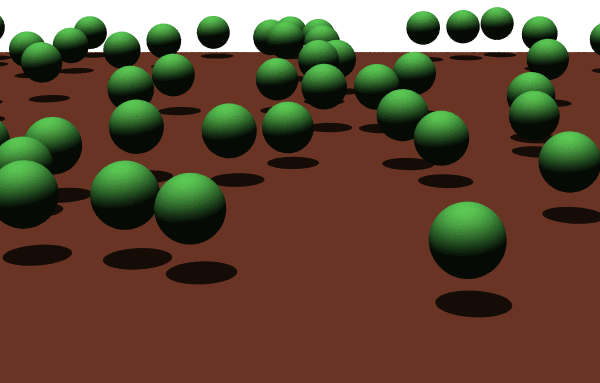
\includegraphics[width=0.33\textwidth]{/home/mn811042/Thesis/chapter4/figures/rami_lai_050.png}}
\subfloat[Medium Canopy]{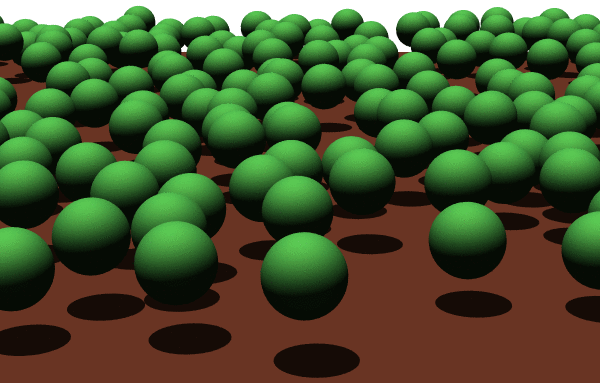
\includegraphics[width=0.33\textwidth]{/home/mn811042/Thesis/chapter4/figures/rami_lai_150.png}}
\subfloat[Dense Canopy]{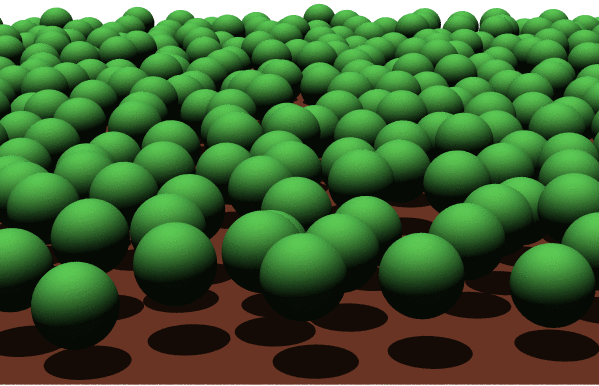
\includegraphics[width=0.33\textwidth]{/home/mn811042/Thesis/chapter4/figures/rami_lai_250.png}}
\end{tabular}
\caption{Graphical representation of the open forest canopy environments used in RAMI4PILPS. The images represent three different canopy structures extracted from \citet{Widlowski2011}.} 
\label{fig:rami}
\end{figure}


\begin{threeparttable}
\centering
\caption{Summary of variables defining structurally heterogeneous scenes (see \citet{Widlowski2011} for details). Different soil albedos are defined as BLK = black, MED = medium, SNW = snow.}
%\begin{tabular*}{\textwidth}{ l@{\extracolsep{\fill}}*{4}{c}}
\begin{tabular}{l{0.25\textwidth} l{0.75\textwidth}}
%\begin{tabular}{\textwidth}{|p{\textwidth/4}|p{\textwidth/4}|p{\textwidth/4}|p{\textwidth/4}|}
%\begin{tabular*}
     \hline
     \hline
\textbf{Variable Identification}   & \textbf{Values (Units)}\\
\noalign{\smallskip}\hline
Leaf Area Index/ canopy	                & 0.50$^S$, 1.50$^M$ and 2.50$^D$ (m$^2$.m$^{-2}$)\\
Leaf Area Index/ sphere	                & 5.0$^S$, 5.0$^M$ and 5.0$^D$  (m$^2$.m$^{-2}$)\\
1 - $P_{gap} (\theta = 0^{\circ})$      & 0.09$^S$, 0.26$^M$ and 0.434$^D$\\
Tree density                            & 12.80$^S$, 38.24$^M$ and 63.68$^D$ (trees/hectare)\\
Maximum canopy height                   & 16 m\\
Minimum sphere centre height	        & 7 m\\
Maximum sphere centre height	        & 11 m\\
$\alpha_{soil}$,PAR / $\alpha_{soil}$,NIR	& BLK: 0.00/0.00; MED: 0.12/0.21; SNW: 0.96/0.56\\
Soil scattering law	                & Lambertian\\
$\rho_{leaf}$,PAR / $\rho_{leaf}$,NIR     & 0.0735/0.3912\\
$\tau_{leaf}$,PAR / $\tau_{leaf}$,NIR     & 0.0566/0.4146\\
Leaf scattering law                     & Bi-Lambertian\\
Sun zenith angle	                & 27.5$^{\circ}$/60.0$^{\circ}$/83.5$^{\circ}$/Isotropic(ISO)\\
Scatterer Normal Distribution           & Spherical\\
Woody area index                        & 0.0 (m$^2$.m$^{-2}$)\\
\hline
\hline%\noalign{\bigskip}
%\end{tabular*}
\end{tabular}
\begin{tablenotes}
      \small
      \item $^S$Sparse vegetation. $^M$Medium vegetation. $^D$Dense vegetation. 
\end{tablenotes}
\label{tab:RAMI4PILPS}
\end{threeparttable}
\bigskip

\section{Modelling photosynthesis with JULES: the Farquhar model}

The leaf photosynthesis is estimated as the minimum of three assimilation limited rates as proposed by \citet{Farquhar1980}: the Rubisco-limited rate or \textbf{carbon limitation} (W$_c$), the light-limited rate or \textbf{light limitation} (W$_l$), and the carbon compound export limitation for C3 plants or PEP-carboxylase export limitation for C4 plants, referred as the electron \textbf{transport} or \textbf{export limitation} (W$_e$). Further details on the photosynthesis parameterisation in JULES are given in \citet{Clark2011}. Following \citet{Collatz1991,Collatz1992} and \citet{Oleson2010} the leaf photosynthesis (A$_n$, mol m$^{-2}$ s$^{-1}$) is estimated as the minimum of three assimilation limiting regimes:
\begin{enumerate}
 \item Carbon limiting rate:
\begin{equation}\label{eq:wc}
 W_c = \left\{
  \begin{array}{l l}
    V_{cmax}\left(\frac{c_i-\varGamma}{c_i+K_c(1+O_a/K_o)}\right) & 
   \quad \textrm{for C$_3$ plants}\\
    V_{cmax} & 
     \quad \textrm {for C$_4$ plants}
  \end{array}\right.
 \end{equation}
\noindent where V$_{cmax}$ (mol CO$_2$ m$^{-2}$ s$^{-1}$) is the maximum rate of carboxylation of Rubisco, c$_i$ (Pa) is the leaf internal carbon dioxide partial pressure, $\varGamma$ (Pa) is the CO$_2$ compensation point in the absence of mitochondrial respiration, $O_a$ (Pa) is the partial pressure of atmospheric oxygen, and K$_c$ and K$_o$ (Pa) are the Michaelis-Menten parameters for CO$_2$ and O$_2$, respectively. For C$_4$ photosynthesis the carbon limitation imposed here corresponds to the carboxylation process of Rubisco in the bundle sheath cells because the carbon concentration is already high inside the plant celles thanks to pumping mechanisms. Photorespiration is also inhibited in C$_4$ plants, thus W$c$ does not depend on CO$_2$ or O$_2$ concentrations \citep{Collatz1992}.

 \item Light limiting rate:
\begin{equation}\label{eq:wl}
 W_l = \left\{
  \begin{array}{l l}
    \alpha fAPAR \cdot I^{\downarrow} \left(\frac{c_i-\varGamma}{c_i+2\varGamma}\right)  & 
   \quad \textrm{for C$_3$ plants}\\
    \alpha fAPAR \cdot I^{\downarrow} & 
     \quad \textrm {for C$_4$ plants}
  \end{array}\right.
 \end{equation}
\noindent where $\alpha$ is the maximum quantum efficiency of photosynthesis (mol CO$_2$ mol$^{−1}$ PAR), which is regulated by the effect of photorespiration as it is multiplied by the term in brackets to give the effective quantum efficiency in C$_3$ plants. In the case of C$_4$ photosynthesis, $\varGamma$ is close to 0 and the quantum efficiency is independent of intercellular carbon concentration, being equal to its maximum value. fAPAR is given by the two-stream scheme and $I^{\downarrow}$ is the incident PAR at the top of the canopy. fAPAR is calculated separetely between sunlit and shaded leaves, therefore the light limiting rate is different between these two types of leaves. The total light limiting rate per layer is the sum between sunlit and shaded W$_l$ weighted by f$_{sun}$ in Equation~\ref{eq:fsun}.

 \item Export limiting rate:
\begin{equation}\label{eq:we}
  W_e = \left\{
  \begin{array}{l l}
    0.5 V_{cmax} & \quad \textrm{for C$_3$ plants}\\
    2 \times 10^4 V_{cmax}\frac{c_i}{P_{*}} & 
     \quad \textrm {for C$_4$ plants}
  \end{array}\right.
 \end{equation}
\noindent where P$_{*}$ is the surface air pressure (Pa). For C$_3$ plants W$_e$ is the rate of transport of photosynthetic products from the chloroplast to other parts of the plant, and for C$_4$ plants it represents the process of the initial carboxylation by PEPCarboxylase.
\end{enumerate}

Two variables that are often used when calculating photosynthesis limiting rates according to the \citet{Farquhar1980} model are independently calculated in JULES, these a are: the maximum rate of carboxylation of Rubisco (V$_{cmax}$) and the CO$_2$ compensation point in the absence of mitochondrial respiration ($\varGamma$), or the photorespiration compensation point. V$_{cmax}$ at any desired temperature is calculated from the maximum rate of carboxylation of the enzyme Rubisco at 25$^{\circ}$C (V$_{cmax25}$) assuming an optimal temperature range as defined by PFT-specific values of parameters (e.g., T$_{upp}$ and T$_{low}$):
\begin{equation}\label{vcmax_T_eq}
 V_{cmax}=\frac{V_{cmax25i} Q_{10{\_}leaf}^{0.1(T_c-25)}}{\left[1+e^{0.3(T_c-T_{upp})}\right]\left[1+e^{0.3(T_{low}-T_c)}\right]}
\end{equation}
\noindent where T$_c$ is canopy (leaf) temperature and Q$_{10{\_}leaf}$ is a temperature dependent function with default value equals 2. Photosynthetic capacity at each canopy layer \textit{i} is calculated assuming that the reference value varies as:
\begin{equation}\label{eq:vcmax25i}
  V_{cmax25i} = \left\{
  \begin{array}{l l}
    0.0008 n_0 e^{-k_n(\frac{i}{n})} & \quad \textrm{for C$_3$ plants}\\
    0.0004 n_0 e^{-k_n(\frac{i}{n})} & \quad \textrm {for C$_4$ plants}
  \end{array}\right.
 \end{equation}
\noindent with $n_0$ the leaf N concentration at the top of the canopy, $k_n$ a nitrogen profile coefficient estimated to be 0.78 \citep{Clark2011}, $i$ is the canopy layer, and $n$ is the total number of layers with default value equals 10. $\varGamma$ at any desired partial pressure of atmospheric oxygen is give by:
\begin{equation}\label{eq:gamma_ju}
  \varGamma = \left\{
  \begin{array}{l l}
     \frac{O_a}{2 \tau} & \quad \textrm{for C$_3$ plants}\\
      0  & 
     \quad \textrm {for C$_4$ plants}
  \end{array}\right.
 \end{equation}
\noindent with $\tau$ the rubisco specifity for CO$_2$ relative to O$_2$, which varies with temperature according to:
\begin{equation}
 \tau = 2600 Q_{10{\_}rs}^{0.1(Tc-25)}
\end{equation}
\noindent with $Q_{10{\_}rs}$=0.57.
The Michaelis-Menten parameters are also temperature dependent:
\begin{equation}
%\begin{split}
%K_c = 30Q_{10Kc}^{0.1(T_c-25)}
%K_c = 3 \cdot 10^{4} Q_{10Ko}^{0.1(T_c-25)}
%\end{split}
\begin{array}{l l}
K_c = 30Q_{10{\_}Kc}^{0.1(T_c-25)} & \\
K_o = 3 \cdot 10^{4} Q_{10{\_}Ko}^{0.1(T_c-25)} &
\end{array}\right.
\end{equation}
\noindent with $Q_{10{\_}Kc}$ = 2.1 and $Q_{10{\_}Ko}$ = 1.2.

In JULES, The rate of gross photosynthesis is calculated from the Farquhar limiting regimes with a set of quadratic equations, which assure a gradual transition from one limitation to another. 
\begin{equation}\label{quadratic}
\begin{split}
\beta_1 W_p^2-W_p(W_c+W_l)+W_cW_l=0 \\
\beta_2 W^2-W(W_p+W_e)+W_pW_e=0
\end{split}
\end{equation}
\noindent where W$_p$ is the smooth minimum of W$_c$ and W$_l$. Finally, W is the gross photosynthetic rate. The smaller root of each quadratic is selected. The values of the co-limitation coefficients are empirically determined \citep{Collatz1990}, in JULES the values $\beta_1$ = 0.83 and $\beta_2$ = 0.93 are used. 

The multi-layer approach for light interception and photosynthesis simulates competition between light and carbon-limited regimes at each canopy layer, resulting
in increased Rubisco limitation towards the top of the canopy and increased light limitation lower in the canopy \citep{Clark2011}.

\section{FLUXNET dataset}

FLUXNET, a ``network of regional network'', is a global network of micrometeorological tower sites that measure the exchange of carbon dioxide, water vapour and energy between the biosphere and atmosphere across a range of biomes and timescales \citep{Baldocchi2001}. Data and site information are available online at: \url{http://www.fluxnet.ornl.gov/}. Over 500 tower sites are located worldwide on five continents and are used to study a range of vegetation types, such as temperate conifer and broadleaved (deciduous and evergreen) forests, tropical and boreal forests, crops, grasslands, wetlands, and tundra \citep{Baldocchi2001}.
%Local observations of GPP were obtained from the FLUXNET network.
Flux tower sites use the eddy covariance method to measure net ecosystem exchange (NEE), which is defined as the net flux of CO$_2$, and is separated into GPP and ecosystem respiration with a ``flux-partitioning algorithm'' \citep{Reichstein2005}.

%There are a number of approaches used to separate NEE into its two component fluxes, which include extrapolating night-time respiration measurements to the daytime and fitting light-response curves to daytime NEE measurements (Lasslop et al., 2010). In addition to flux-partitioning, the data must also be gap-filled due to unfavourable meteorological conditions and instrument failure (Reichstein et al., 2005). These processes carry with them some uncertainty, which must be quantified. Hagen et al. (2006) found that the uncertainty at the half-hourly timescale was of the order of the observations themselves (i.e. ∼ 100\%), but only ∼ 10\% at the annual timescales for a temperate deciduous forest.

\section{Study sites}

\subsection{Boreal forests: the BOREAS sites}

The BOREAS Project was set on the Northern and Southern edges of the Canadian boreal forest in a 1000 x 1000 km region covering most of Saskatchewan and Manitoba, Canada. The BOREAS Science Steering Committee conducted the initial study area selection in 1990. This work was followed up by BOREAS staff visits in 1991, 1992 and 1993. The finalised study areas are: 1) Northern Study Area: An area of 8000 square km, located between Thompson Manitoba and Nelson House Manitoba in which five tower flux sites are located within the area, and three of these were used in the present study:
\begin{enumerate}[i]
 \item) Northern Study Area - Old Black Spruce Site (NSA-OBS): The Old Black Spruce site contained a large 30 meter flux tower that topped out in the canopy of large spruce trees over a wet soil.
 \item) Northern Study Area - Old Jack Pine Site (NSA-OJP): The Old Jack Pine site contained a large flux tower, an meteorological tower over dry soil.
 \item) Northern Study Area - Young Jack Pine Site (NSA-YJP): This site was located in a large area of young jack pines, all only about 2 meters high. This is the result of a fire in the area around 1984. Jack Pine cones are sealed shut by sap, and it is only the intense heat of fire that boils the sap and causes the cones to pop open, thus releasing the seeds onto the newly burned, enriched, and dry soil.
\end{enumerate}
2) Southern Study Area: For the Southern Study Area, it proved to be difficult to find extensive stands of the required cover types grouped together in one locale. As a result, the six TF sites are distributed over the area of Prince Albert National Park through to the Candle Lake Saskatchewan and surrounding area covering a total area of 11170 square km. Four of these study sites were used in the present study:
\begin{enumerate}[i]
 \item) Southern Study Area - Old Black Spruce Site (SSA-OBS): The southern Old Black Spruce site was equipped with a 25 meter double-scaffold tower (with internal steps) extending 5 m above the forest canopy. Screw anchors for tower foundations and guy-wire anchors had to be drilled into the mineral soil beneath a one-meter deep mat of sphagnum moss.
 \item) Southern Study Area - Old Jack Pine Site (SSA-OJP): The Southern Old Jack Pine site contained a large scaffold-style flux tower, linked by cables to a thinner truss tower 100 meters away. There was an under-canopy radiation sensor mounted on a movable cart on a track running under the trees. There was also a large canopy access tower to allow scientists to get direct acess to the canopy for experiments. 
 \item) Southern Study Area - Young Jack Pine Site (SSA-YJP): The Young Jack Pine site is located just south of the Narrow Hills Provincial Park, west of Route 106. It has a small truss-style flux tower down a small trail from the hut.
 \item) Southern Study Area - Old Aspen Site (SSA-OA): This site is located within the boundaries of Prince Albert Provincial Park, and is accessed by a long trail. It has a large scaffold flux tower (with a truss tower connected by cables), a small 4 meter under canopy flux tower (south of huts), two canopy access towers, a SRC meteorological tower, and a tethered balloon with a radiosonde.
\end{enumerate}

\begin{figure}[ht!]
\centering
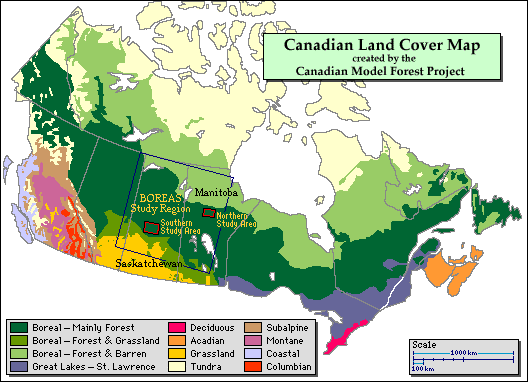
\includegraphics[width=0.75\textwidth]{/home/mn811042/Thesis/chapter3/figures/BOREAS_Canada_Forest_Map3.png}
\caption{Land Cover map of Canada showing the BOREAS Study Region and the Northern and Southern Sites. From: \url{https://daac.ornl.gov/BOREAS/bhs/Study_Region.html}} 
\label{f:boreas_plot}
\end{figure}

Hemispherical photographs were acquired in sample arrays at heights of 0.8, 1.5, and 2.5 m for each of the forested BOREAS tower flux sites and auxiliary sites. For the forested tower flux sites and other sites for which mapped plots were set up, hemispherical photographs were acquired during IFC-1 and IFC-2 at 10 m intervals along the central X axis of the mapped plot (5 m intervals for NSA-YJP). Typically, this corresponds to six sample locations for each tower flux site. Site locations in relation to the flux tower are SSA-OBS, 150-230 m (SE); SSA-OJP, 130-180 m (SE); SSA-YJP, 30-80 m (SE); SSA-OA, 70-120 m (SW); NSA-OBS, 80-130 m (SE); NSA-OJP, 70-120 m (SE); and NSA-YJP, 120-150 m (SE). %Location refers to distance from the flux tower along the ``B'' LAI transect, except in the case of SOBS, where a ``D'' line (20 m from the C line) is used. For the auxiliary sites, hemispherical photographs were taken in a crisscross array, at 10 m intervals along two 40 m long transects placed at right angles and crossing in the middle. A total of nine sample locations were chosen within the plot. The auxiliary site photographs were taken during and between IFC-1 and IFC-2.
Hemispherical photograph negatives were video digitized at a resolution of 512 (horizontal) x 480 (vertical) x 7 bits using the hemispherical photograph analysis system CANOPY \citep{Rich1989,Rich1990}. Gap fraction, the proportion of unobstructed sky, was calculated at 5$^{\circ}$ zenith angle intervals and used for additional calculations. All hemisphericai photographs were also archived in Kodak PhotoCD format. The effective LA1 and other canopy indices were calculated using the program LAICALC \citep{Rich1995} following the method of \citet{Chen1991}. In order to compare hemispherical photography technique and LAI-2000 results, the gap fractions from the photographs were similarly separated into five zenith angles from 0 to 75$^{\circ}$.

\subsection{Temperate conifereous forest: Oregon sites}

The Oregon sites encompass two broad forest age classes: i) mature with tree age ranging from 95 to 316 years (US-Me4), and intermediate with tree age ranging from 56 to 89 years (US-Me2) \citep{Law2003}. The study area is located east of the Cascades Range and its position relative to the coast and mountains creates a semi-arid climate; annual precipitation is between 350 and 880 mm \citep{Law2001,Williams2005,Dekauwe2011}. 
The mature study area (44.4992$^{\circ}$N, 121.6224$^{\circ}$W) was located within the Metolius Research Natural Area (RNA) and the Metolius river basin and is characterised primarily by an old growth coniferous pine forest. The mature site is dominated by ponderosa pine (\textit{Pinus ponderosa}) and to a lesser extent grand fir (\textit{Abies grandis}) and western larch (\textit{Larix occidentalis}) \citep{Dekauwe2011}. The site is very open and is in fact a mixture of old-growth (95-316 years), mixed age (56-89 years) and young trees ($<$ 23 years). Older-growth trees are free of foliage on the lower section of their stems, partly due to light competition and/or fire, with limited understory foliage. The understory species present are a small scattering of bracken fern (\textit{Pteridium aquilinum}) and strawberries (\textit{Fragaria vesca}). 
The intermediate (44.4524$^{\circ}$N, 121.5572$^{\circ}$W) sites are located on a section of privately owned land and had previously been old-growth forest that was cleared and allowed to regenerate naturally \citep{Schwarz2004}. \citet{Schwarz2004} report that the average stand age in the intermediate site is now approximately
90 years old and that the young site was felled in 1978, then left to regenerate. Both sites can largely be characterised by ponderosa pine and incense-cedar (\textit{Calocedrus decurrens}) with a large ($\approx$ 0.51 m) understory of Manzanita (\textit{Arctostaphylos patula}), and Bitterbush (\textit{Purshia tri-dentata}). Both sites maintain, or previously maintained flux towers and are part of the AmeriFlux network of flux towers, with CO$_2$ flux measurements recorded at the study sites at periods between 1999 and the present. 

Hemispherical photographs were acquired in the highest non-RAW mode, i.e., fine JPEG, which has a compression factor of 1:4. A tripod was not used as the sampling time window was limited and the aim was to sample widely from as many locations as possible. When taking upward looking photographs, the camera was held at arm's
length and at eye level, with the user leveling the camera by eye across the camera body so that each picture was taken level and in approximately the same position. Carrying out the measurements rapidly in this way allows more than 10× the number of measurements that would be possible where leveling is carried out for each
image acquisition. The small additional uncertainty in the resulting measurements is traded off against a much greater number of measurements across a wide area. The data was acquired and shared by Dr. M.G. De Kauwe, and more details about sampling can be found in \citet{Dekauwe2011}.

%The VALERI approach to obtaining in situ observations \citep{Baret1999} was adopted for this study. The VALERI method involved obtaining a cluster of in situ samples which cover the same spatial extent of representative pixels in a higher resolution satellite image, in this case from three 9 km$^2$ sub-regions defined within a 121 km$^2$ area. Ideally, the area depicted within each of these 9 km$^2$ regions should be relatively homogeneous and representative of the age class. In practice this was difficult, due in part to the topography, but largely because sections of the intermediate and young sites lie on private land and are subject to management. All of the forested areas within the study site are also subject to frequent fire disturbance which promotes a high level of heterogeneity across the landscape as not all of the burning is managed \citep{Law2003}.
%Moreover whilst the three flux towers are erected to sample within a footprint defined to broadly represent a forest age class, the satellite platforms will not be sampling an identical footprint, which is why a 9 km$^2$ area is used to represent satellite observations from nominally 1 km$^2$ pixel (accounting for geolocation errors). The 9 km$^2$ area was divided into nine 1 km$^2$ boxes and within each box, three Elementary Sampling Units (ESU) were defined which are representative of the high resolution satellite pixel. Each ESU was chosen to represent a 30 m pixel so that each pixel could be directly matched to a high resolution (30 m) Landsat ETM+image of the site. ESUs were randomly located within each 1 km$^2$ box, so as to reduce bias and sample the natural variability of the landscape. If an ESU was found to lie on a road or at an inaccessible location then it was randomly relocated to a nearby location 100 m away. If this new location was also inaccessible the methodology was carried out again or until a suitable location was obtained. The central 1 km$^2$ box was more intensively sampled as it represents the intended focus of the satellite observation. Five ESUs were defined within this box and a transect dissecting the central box was also sampled (100 measurements).
%Additionally, seventeen further ESUs were defined using a stratified random sampling scheme across the 121 km$^2$ area to sample locations not covered by the three 9 km$^2$ grids. Where possible, additional ESUs were defined, resulting in four extra plots at the mature site and a further ESU at the intermediate site. Employing this method resulted in 1284 LAI measurements from 107 ESU plots across the study area, excluding the transect measurements.
%Error of individual in situ samples was not assessed due to cost and time constraints. However, \citet{Williams2005} suggest relative errors of 10\% for in situ samples taken from the LAI-2000 for the same site \citep{Law2001}.

\subsection{Woody-savannah: Tonzi Ranch}

Tonzi Ranch (latitude: 38.4318$^{\circ}$N; longitude: 120.9668$^{\circ}$W; altitude: 177 m) is located in the lower foothills of the Sierra Nevada Mountains, Ione, CA, USA, and it is part of the AmeriFlux (\url{http://public.ornl.gov/ameriflux/}). It is classified as an oak-grass savanna woodland on flat terrain (average slope: 1.58$^{\circ}$), and experiences Mediterranean-type climate with dry, hot summers and rainy, mild winters. Annual average temperature and annual precipitation are 16.9$^{\circ}$C and 565 mm, respectively (1949 - 2005 climate normals from Camp Pardee climate station; latitude; 38.258$^{\circ}$N; longitude: 120.858$^{\circ}$W). The overstory consists of dominant blue oak trees (\textit{Quercus douglasii}) with occasional ($<$10\%) grey pine trees (\textit{Pinus sabiniana}). The understory is mainly composed of grasses and forbs (\textit{Brachypodium distachyon}, \textit{Hypochaeris glabra}, \textit{Bromus madritensis}, \textit{Cynosurus echinatus}) \citep{Baldocchi2004}. Due to the low density of grey pine trees (\textit{Pinus sabiniana}), it is assumed no element clumping (related only to needle-to-shoot strcuture). The stem density was 144 ha$^{-1}$, tree height was 9.4 $\pm$ 4.3 m (mean $\pm$ standard deviation), trunk height was 1.8 $\pm$ 1.3 m, diameter at breast height (DBH) was 0.26 $\pm$ 0.11 m, mean crown radius was 2.9 $\pm$ 1.4 m, and canopy cover was 0.47 \citep{Chen2008}. More detailed site information may be found in previous studies \citep{Baldocchi2004,Ma2007,Chen2008}. DHPs were acquired by \citet{Ryu2010} from 5$^{th}$ to 7$^{th}$ of August, 2008, close to the peak of the growing season, on a 300 m $x$ 300 m sampling plot with the flux tower at the centrer, gridded at 30 m $x$ 30 m intervals. The extent of the plot corresponds to the scale of spatial heterogeneity as determined through semivariogram analysis \citep{Kim2006}.

%Direct transmissivity was extracted from the DHPs using the CIMES-FISHEYE software \citep{Walter2012}. First, the raw photographs were oriented to the geographic North; East and West are inverted on Hemispherical Photographs (East left, West right). Second, the horizon circle of the image have to be identified, and to do so, brightness should be increased, and contrast adjusted. Third, the pixel coordinates of 3 points clearly defined on the inner border of the circle are enough to describe the hemisphere of the photograph. The coordinates are used in the software to centre the image and define its circular limit. For this set of DHPs, there was no need to repeat this procedure for other images, since their position and diameter did not vary from one image to the next. Fourth, colour digital images are made of pixels, and pixels are made of combinations of primary colours. A channel in this context is the grayscale image of the same size as a colour image, made of just one of the primary colours. For instance, an image from a standard digital perspective will have a red, a green, and a blue channel, or RGB. A grayscale image has just one channel. The green channel translates best halftones but is not suited for analysis. The red and blue channels offer good contrast separating sky (background) from plants (foreground). Usually for analysis, the blue channel is selected (Figure~\ref{f:bluepic}) and the remaining channels are discarded. 

%Fifth, the selection of an appropriate method to calculate a threshold is of concern to hemispherical photography analysis. Some softwares offers several methods to determine automatically a global threshold value derived from the histogram of grey levels of the whole image \citep{Ridler1978}. In fact, there is no perfect thresholding method, therefore, to ensure consistency, it is important to always use the same method for a given set of photographs. It allows repeatability of the process, independent of any user. For Tonzi Ranch the chosen threshold was globally set to 195. However, under bright light conditions, the threshold was increased, and under dark light conditions the threshold was decreased. Within 52 photographs, 12 presented abnormal light condition (either too bright, or too dark). The other 40 photographs were set at 195 threshold. The final step is converting the grey-toned image to a binary (classified) image, where black pixels represent foliage and white pixels sky.

\subsection{Mixed Forest: Alice Holt}

Alice Holt forest is currently dominated by Corsican pine (\textit{Pinus nigra}) but 140 hectares of older oak (\textit{Quercus robur}) woodland remain. Currently, the oldest oak stands are comprised of trees over 180 years of age, and it has a well developed vernal ground flora and a shrub layer. Climate is typical of south-east England with a growing season from mid March to early November. Annual average temperature is 10.1$^{\circ}$C and mean annual rainfall is 779 mm \citep{Benham2012}. Hemispherical photos were taken in August 2015, 15$^{th}$ and 16$^{th}$ by Ewan Pinnington.

\subsection{Temperate conifereous forest: Harvard Forest Hemlock site}

The hemlock-dominated forest (42.47$^{\circ}$N, 72.22$^{\circ}$W, altitude 200m) occupies about 7 ha with trees ranging in age from 100 to around 230 years. This forest was never cleared for agriculture, although selected trees were removed from the stand during the 19$^{th}$ century and in the early 20$^{th}$ century . The hemlock-dominated forest occupies about 7 ha and it is bordered by forests dominated by red oak (\textit{Quercus rubra L.}) and red maple (\textit{Acer rubrum L.}), with scattered white pine (\textit{Pinus strobus L.}) to the north and east, and a red pine (\textit{Pinus resinosa Ait.}) plantation to the south. A bog with red spruce (\textit{Picea rubens Sarg.}), black gum (\textit{Nyssa sylvatica L.}) and red maple (\textit{Acer rubrum L.}) is located west of the hemlock stand. Because of its proximity to the bog and water table, the hemlock forest is unlikely to suffer persistent water stress \citep{Hadley2002}.
The light reaching the forest floor is measured annually in spring (leaf-off) and summer/autumn (leaf-on) using hemispherical photographs since 2004. Every 15 m in each of the 8 experimental plots in the Simes Tract, a photograph of the canopy is taken using a Nikon 8mm fish-eye lens mounted on a Nikon F3 (non-digital) camera. The camera is mounted on a tripod and positioned 1-2 m above ground. The camera is leveled (using self-leveling gimbals) and oriented with magnetic north at the top of the negative \citep{Ellison2005}.
Leaf area index is measured with the LAI-2000 canopy analyzer. Data are collected under diffuse-light conditions, either around the time of sunrise or in cloudy weather, with one LAI sensor continuously logging data above the canopy on an eddy flux tower, and measurements with the other sensor made at multiple plots within each forest type - usually 12 plots within the old-growth hemlock forest \citep{Orwig2009}

\section{Global experiment setup}

\subsection{Model description and experimental design}

For the JULES model global simulations, the version 4.6 was run offline at 0.5$^{\circ}$ x 0.5$^{\circ}$ spatial resolution forced with the 3 hourly WFDEI dataset \citep{Weedon2014} for the year of 2008. The WFDEI dataset contains the following meteorological variables: downward shortwave and longwave radiation fluxes (W m$^{-2}$), rainfall rate (kg m$^{-2}$ s${-1}$), snowfall rate (kg m$^{-2}$s$^{-1}$), 2 m temperature (K), 10 m wind speed (m s$^{-1}$), surface pressure (Pa), and 2 m specific humidity (kg kg${-1}$). The WFDEI dataset has two precipitation products, corrected using either CRU (Climate Research Unit at the University of East Anglia) or GPCC (Global Precipitation Climatology Centre) precipitation totals \citep{Weedon2014}, the so-called WFDEI-CRU and WFDEI-GPCC, respectively, and for this experiment the product WFDEI-CRU was used. The diffuse shortwave radiation was set to a constant value of 40\% of the downward shortwave radiation flux following \citet{Harper2016}.

As described in Section~\ref{sec:fveg}, JULES gridboxes consist of a mixture of 9 surface types, which 5 are PFTS (broadleaf, needleleaf, C3, C4, and shrub) and 4 are non-vegetated surface types (urban, inland water, bare soilm and ice). These 9 surface types are modelled as 9 tiles specified by PFT fractions for each model gridbox at the global scale following the Global Land Cover Characterization database version 2.0 \citep{Loveland2000}. The model was configured following the Met Office JULES Global Land 4.0 configurations \citep{Walters2014} with the Harmonized World Soil Database version 1.0 soil dataset \citep{Nachtergaele2008} and the model of runoff production (TOPMODEL) following \citet{Clark2008}. Prior to performing the global scale model simulations, the soil moisture and temperature was brought to equilibrium using a 5 year global spin-up by cycling 1 year of meteorological data (2008) with the leaf phenology model on following \citet{Cox2001} and described in \citet{Clark2011} updated every 10 days.

JULES version 4.6 includes a canopy clumping index, which scales LAI within the canopy radiation scheme and represents variation within and across canopy structures \citep{Williams2017}. The canopy structure factor (can$\_$struct$\_$a$\_$io) was added in version 4.6 of JULES with default value 1.0, which indicates a structurally homogeneous canopy. This new variable corresponds to the structure factor ($\zeta(\mu)$) in \citet{pinty2006} except assumed not to vary with zenith angle, i.e., $b$ = 0. The canopy structure factor has no impact on the radiative transfer in JULES if can$\_$rad$\_$mod = 1. The variable was originally implemented in JULES by PFT and it was tested and evaluated over crops by \citet{Williams2017}. The authors found that a clumping index between 0.5 and 0.8 would be consistent with the majority of the canopy structures evaluated in their study. For this present study, the model was modified to include a clumping index not only per PFT, but per PFT per gridbox based on a global map of clumping index derived from MODIS \citep{He2012}.

\subsection{MODIS derived clumping index}

%The importance of addressing canopy structure in fieldwork observations is greatly appreciated by the scientific community. There are several distinct methods to obtain structural patterns from vegetation with their specific qualities and limitations. For example, 

Satellite observations are a valid tool to estimate biogephysical parameters from vegetation over very large areas, usually the whole globe. However, the resolution of these variables are limited to the satellite pixels, which are usually not directly comparable to measurements acquired in-situ. In the case of clumping index, \citep{Chen2005} used the bidirectional reflectance distribution function (BRDF) of vegetated land surfaces to extract vegetation structural information globally, using multi-angular data from the POLDER instrument. For the first time, a global clumping index map was derived assisted by a geometrical optical model. However, the clumping index map presented by these authors has several limitations, as low spatial resolution (7 km resolution), topographic effects, and a lack of evaluation with field measurements. Later on, further studies from the same research group improved and validated the global clumping index map with in-situ observations \citep{Pisek2010}.

Using BRDFs, \citet{He2012} derived for the first time a global clumping index map at 500 m resolution from MODIS (Moderate Resolution Imaging Spectroradiometer). However, MODIS-derived clumping index map was found to be consistently lower than available ground data, and it has no zenith angular dependency. Following the same research questions and deriving a clumping index map from MISR data \citep{Pisek2013}, \citet{Pisek2015} developed a comparison study between all available satellite based clumping index products and in-situ observations. Among their main conclusions, the authors pointed out for the fact that the MODIS clumping index map \citep{He2012} with its spatial resolution at 500 m compared to 6 km from POLDER might be more suitable for use in LSMs given the spatial resolution, and that correct land cover information (broadleaf vs. needle-leaf) is crucial for retrieving accurate clumping index values.
%Furthermore, satellite sensors cannot provide correct clumping index estimates over areas with insufficient vegetation coverage ($<$ 25\%), i.e., sparse canopies.

In order to generate a global clumping index map per PFT at a lower resolution compatible with JULES, the GLC-2000 land cover map \citep{Bartholome2005} was used to relate 23 different land cover types into 5 PFTs in JULES according to Table~\ref{tab:glc2000_ci}. The GLC-2000 land cover was used to determine the canopy crown shapes, which are required by the algorithm of \citet{Chen2005} used to generate the MODIS-derived global clumping index map. 

\begin{threeparttable}[ht!]
\centering
\caption{GLC-2000 land cover type to JULES PFTs used to generate global map of MODIS-derived clumping index in 0.5$^{\circ}$ resolution for 2006 based in \citet{He2012}.}
%\begin{tabular*}{\textwidth}{ l@{\extracolsep{\fill}}*{4}{c}}
\begin{tabular}{l{0.25\textwidth} l{0.75\textwidth}}
%\begin{tabular}{\textwidth}{|p{\textwidth/4}|p{\textwidth/4}|p{\textwidth/4}|p{\textwidth/4}|}
%\begin{tabular*}
     \hline
     \hline
\textbf{GLC-2000 land cover}   & \textbf{JULES PFT}\\
\noalign{\smallskip}\hline
Tree Cover, broadleaved, evergreen                       & Broadleaf\\ 
Tree Cover, broadleaved, deciduous, closed               & Broadleaf\\
Tree Cover, broadleaved, deciduous, open                 & Broadleaf\\
Tree Cover, needle-leaved, evergreen                     & Needle-leaf\\
Tree Cover, needle-leaved, deciduous                     & Needle-leaf\\
Tree Cover, mixed leaf type                              & Broadleaf\\
Tree Cover, regularly flooded, fresh  water              & Broadleaf\\
Tree Cover, regularly flooded, saline water              & Broadleaf\\
Mosaic: Tree cover / Other natural vegetation            & Broadleaf\\
Tree Cover, burnt                                        & Broadleaf\\
Shrub Cover, closed-open, evergreen                      & Shrub\\
Shrub Cover, closed-open, deciduous                      & Shrub\\
Herbaceous Cover, closed-open                            & C3\\
Sparse Herbaceous or sparse Shrub Cover                  & C3\\
Regularly flooded Shrub and/or Herbaceous Cover          & C3\\
Cultivated and managed areas                             & C4\\
Mosaic: Cropland / Tree Cover / Other natural vegetation & C4\\
Mosaic: Cropland / Shrub or Grass Cover                  & C4\\
Bare Areas                                               & \textit{NA}\\
Water Bodies                                             & \textit{NA}\\
Snow and Ice                                             & \textit{NA}\\
Artificial surfaces and associated areas                 & \textit{NA}\\
No data                                                  & \textit{NA}\\
\hline
\hline%\noalign{\bigskip}
%\end{tabular*}
\end{tabular}
\begin{tablenotes}
      \small
      \item \textit{NA}: Not applicable. 
\end{tablenotes}
\label{tab:glc2000_ci}
\end{threeparttable}
\bigskip

\begin{figure}[ht!]
\centering
\subfloat[Gridbox]{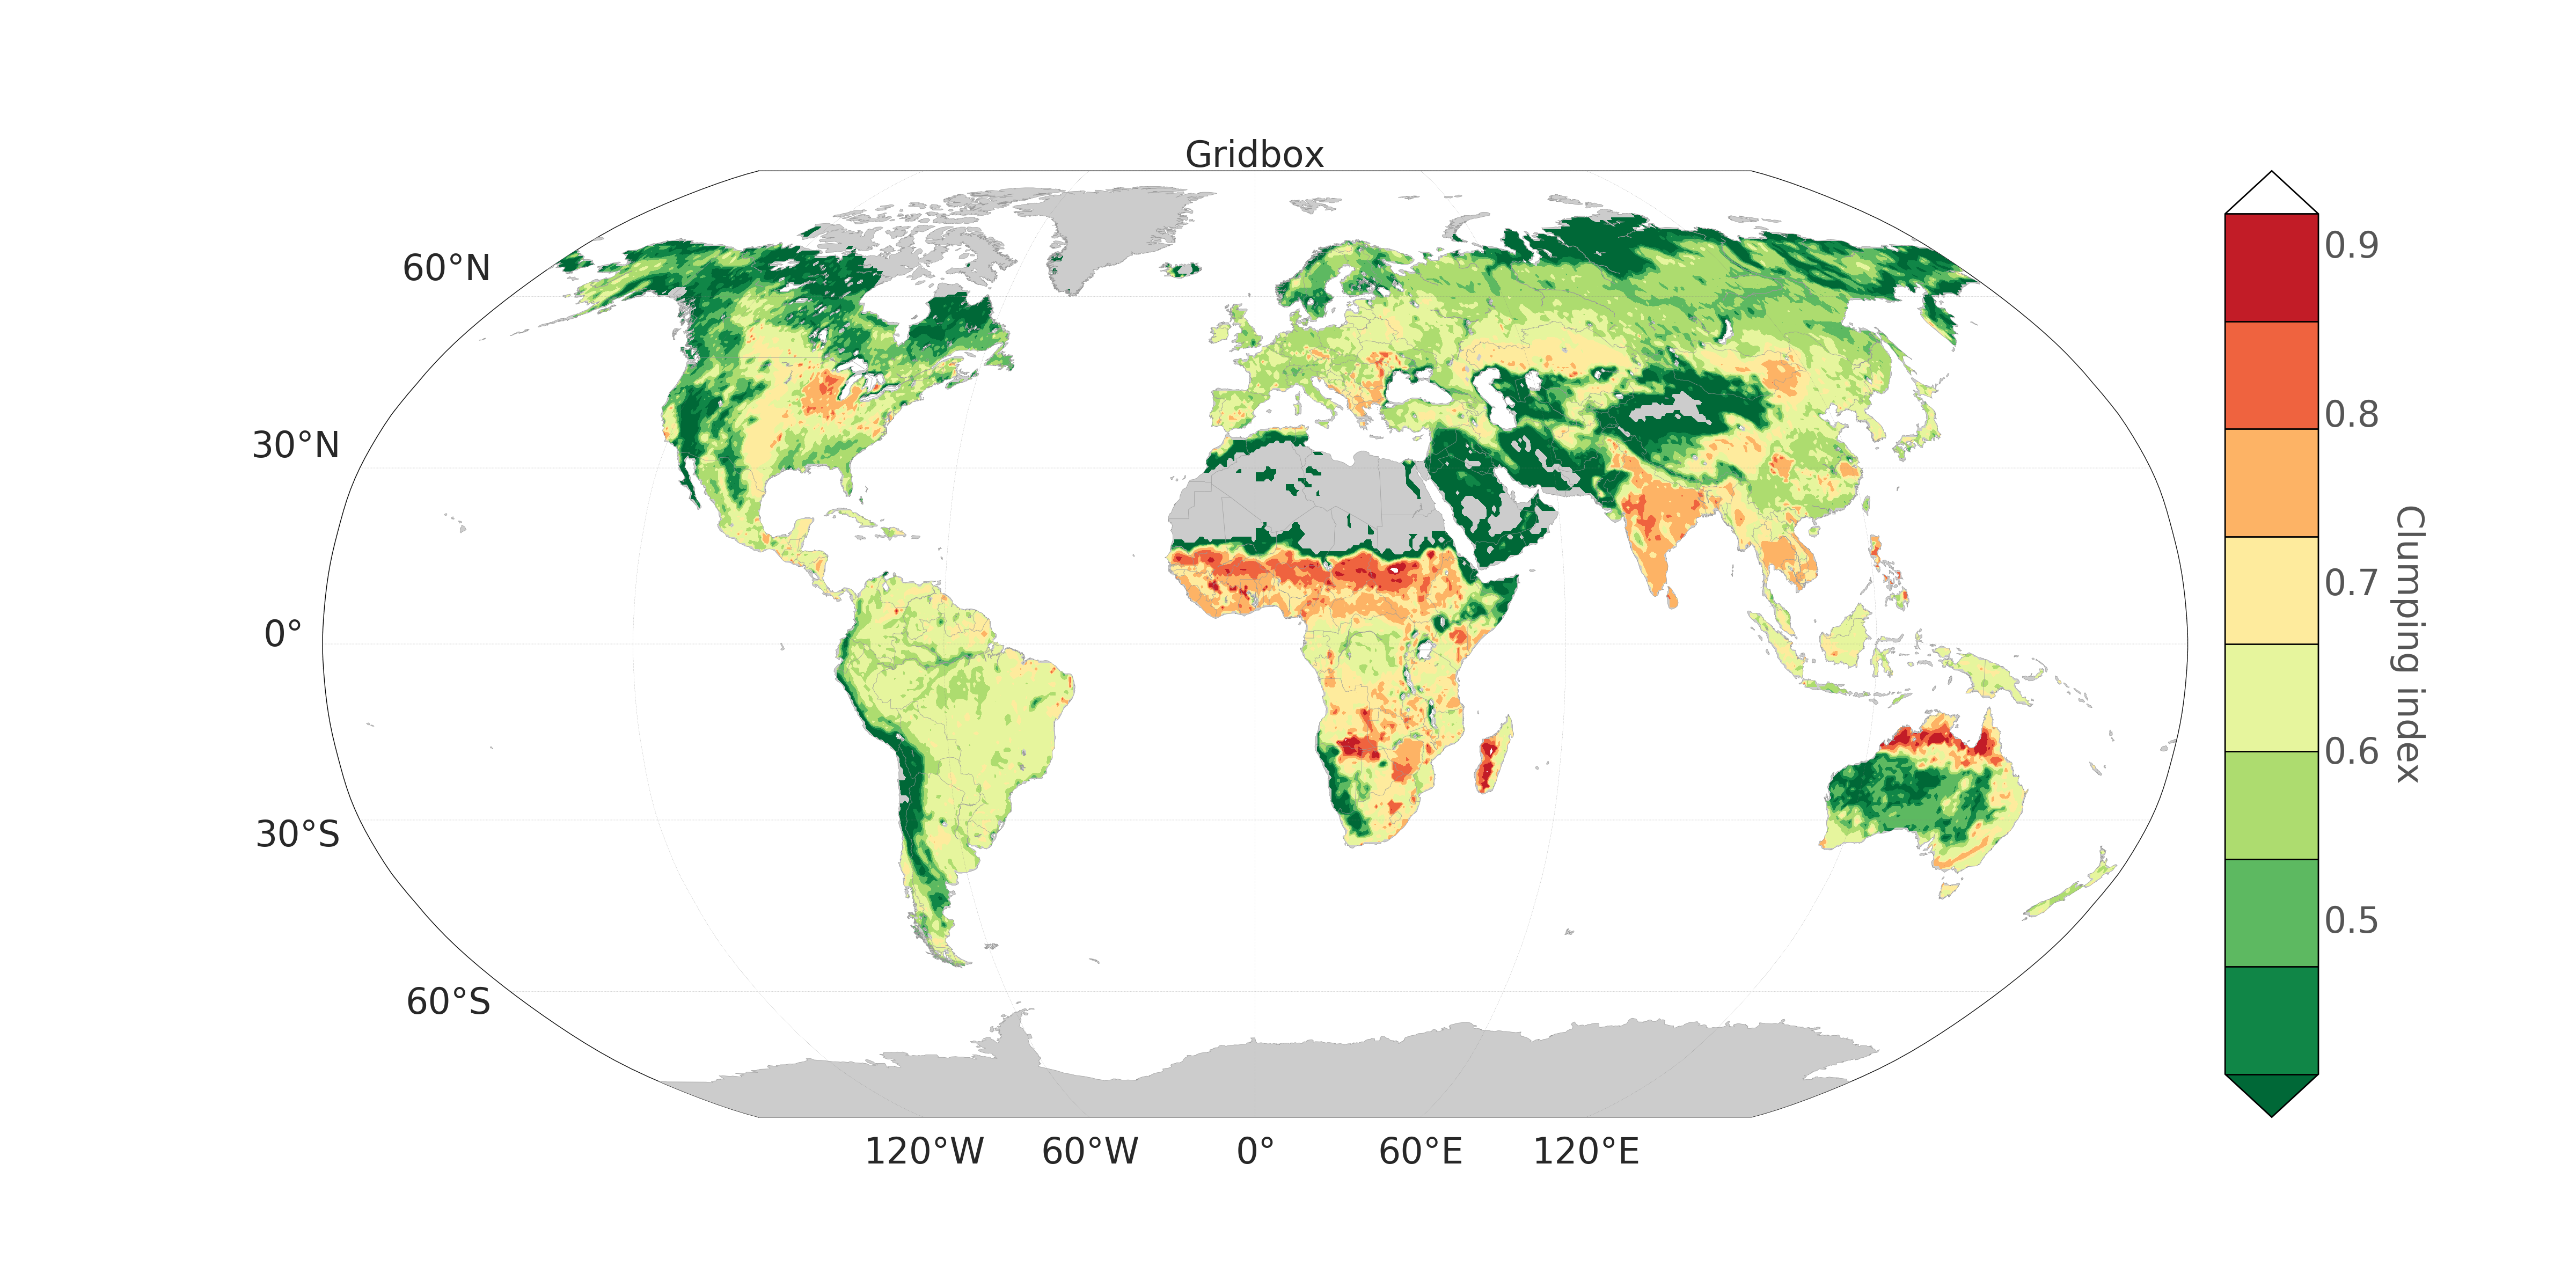
\includegraphics[width=1.0\textwidth]{/home/mn811042/Thesis/chapter6/figures_ofi/clump_PFT_5.png}}
\begin{tabular}{ll}
\subfloat[BL]{\includegraphics[width=0.5\textwidth]{/home/mn811042/Thesis/chapter6/figures_ofi/clump_PFT_0.png}}
\subfloat[NL]{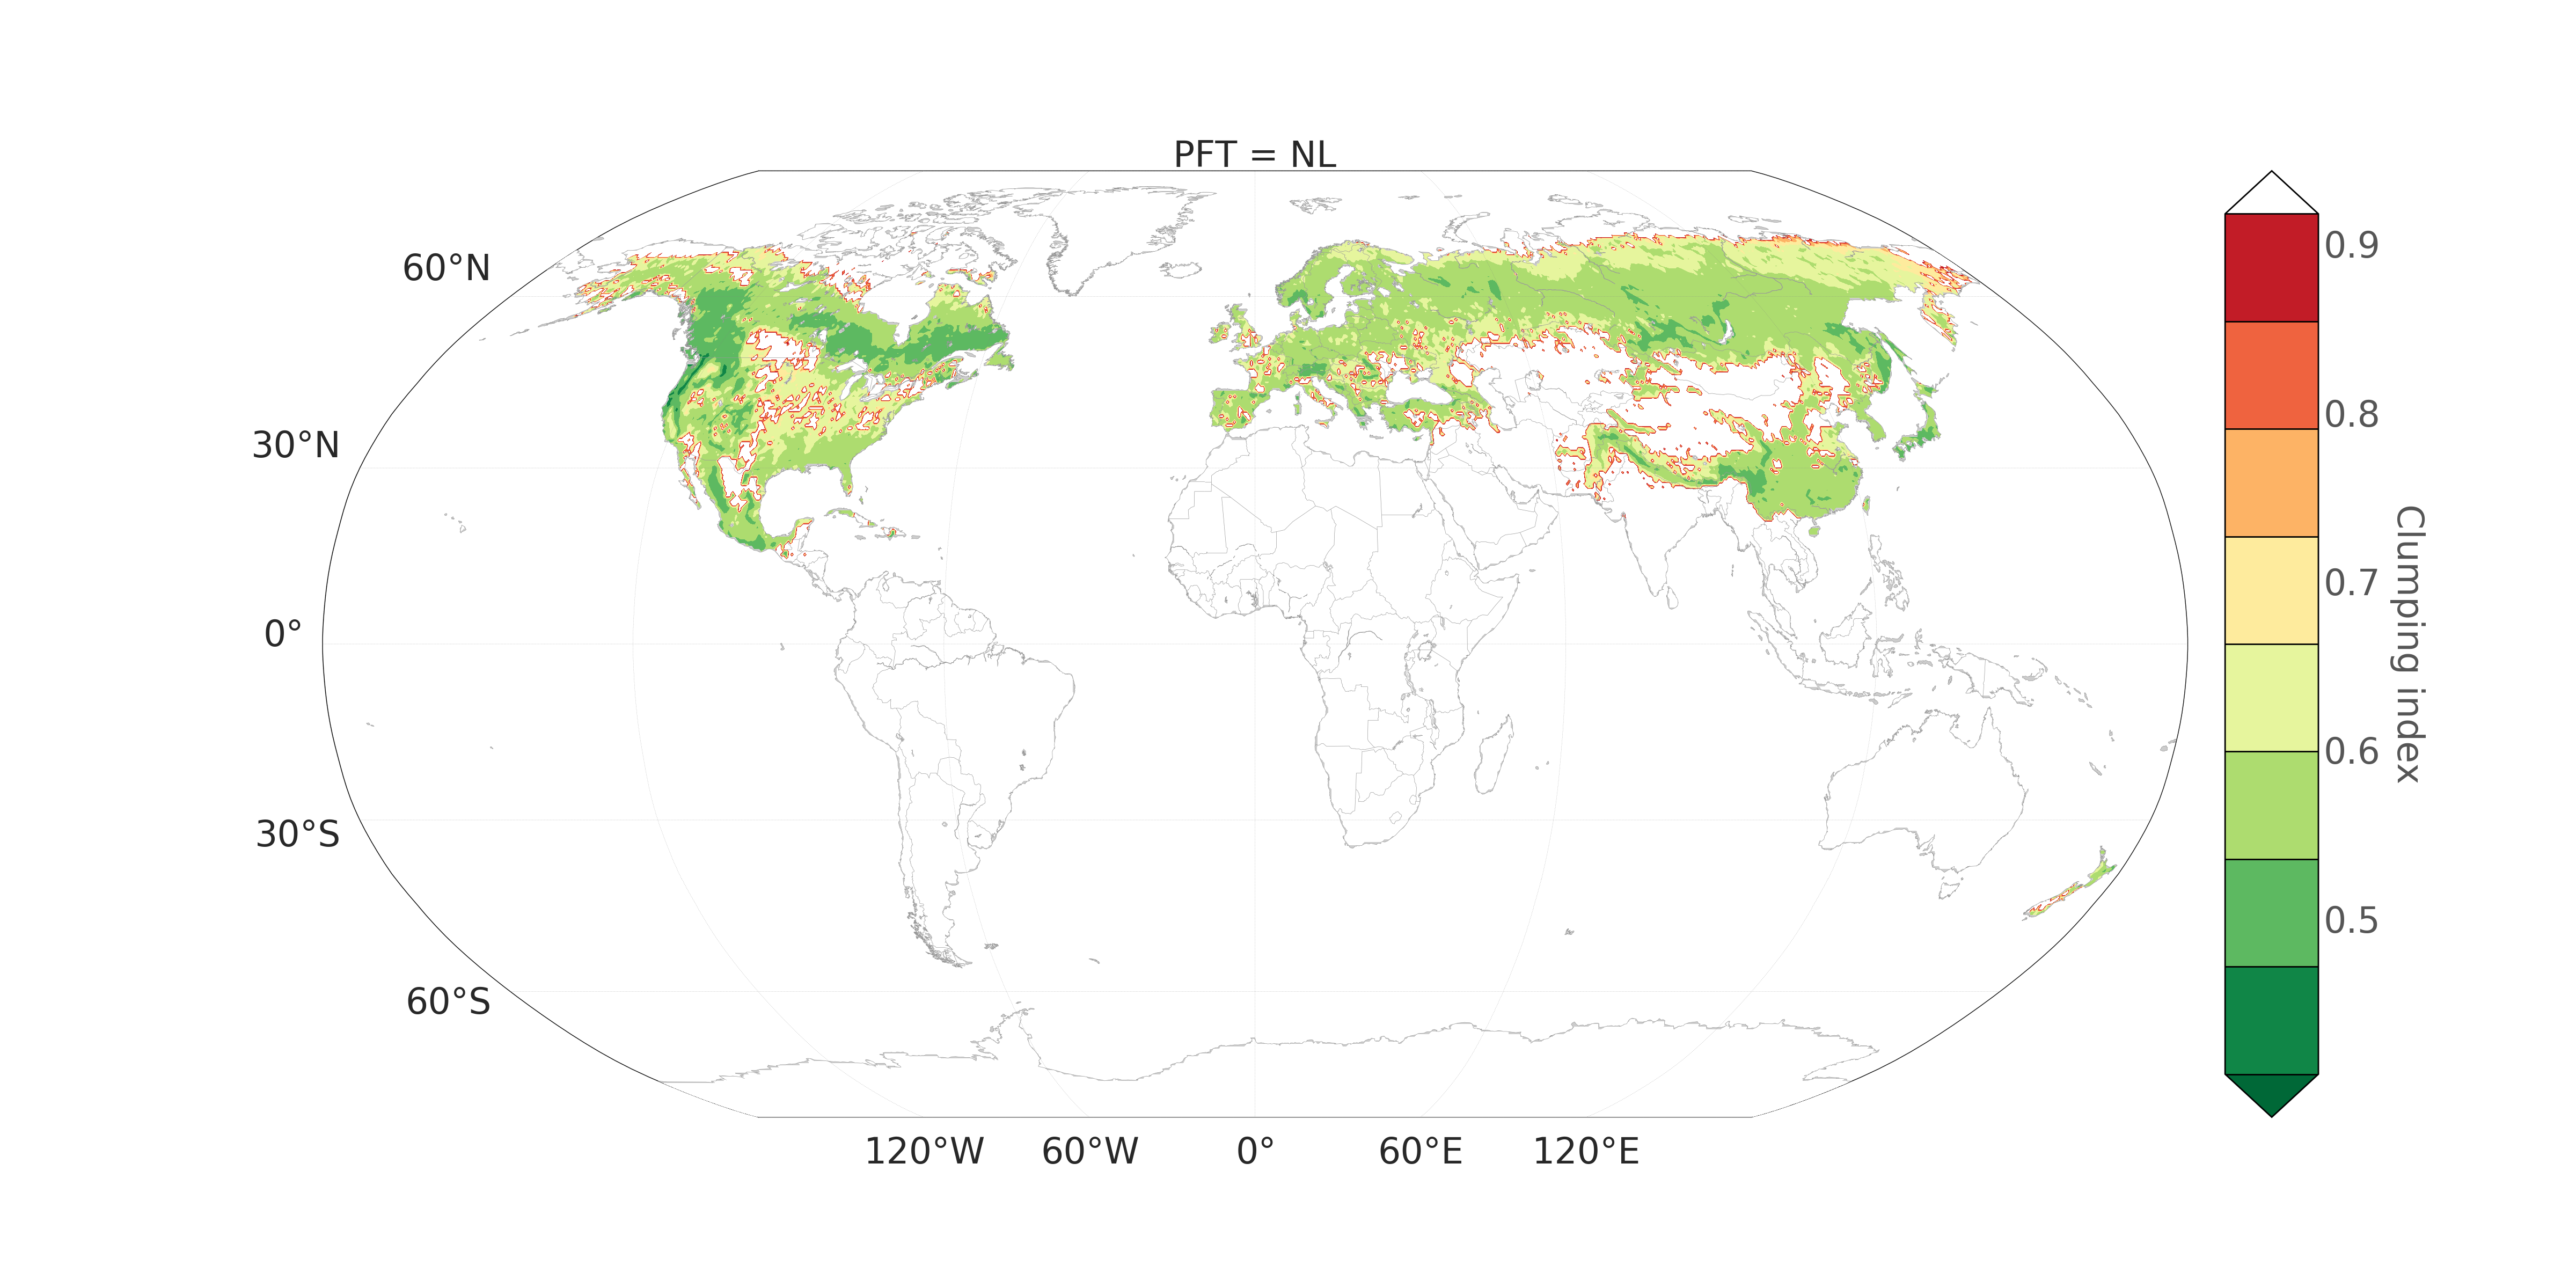
\includegraphics[width=0.5\textwidth]{/home/mn811042/Thesis/chapter6/figures_ofi/clump_PFT_1.png}}
\end{tabular}
\begin{tabular}{ll}
\subfloat[C3]{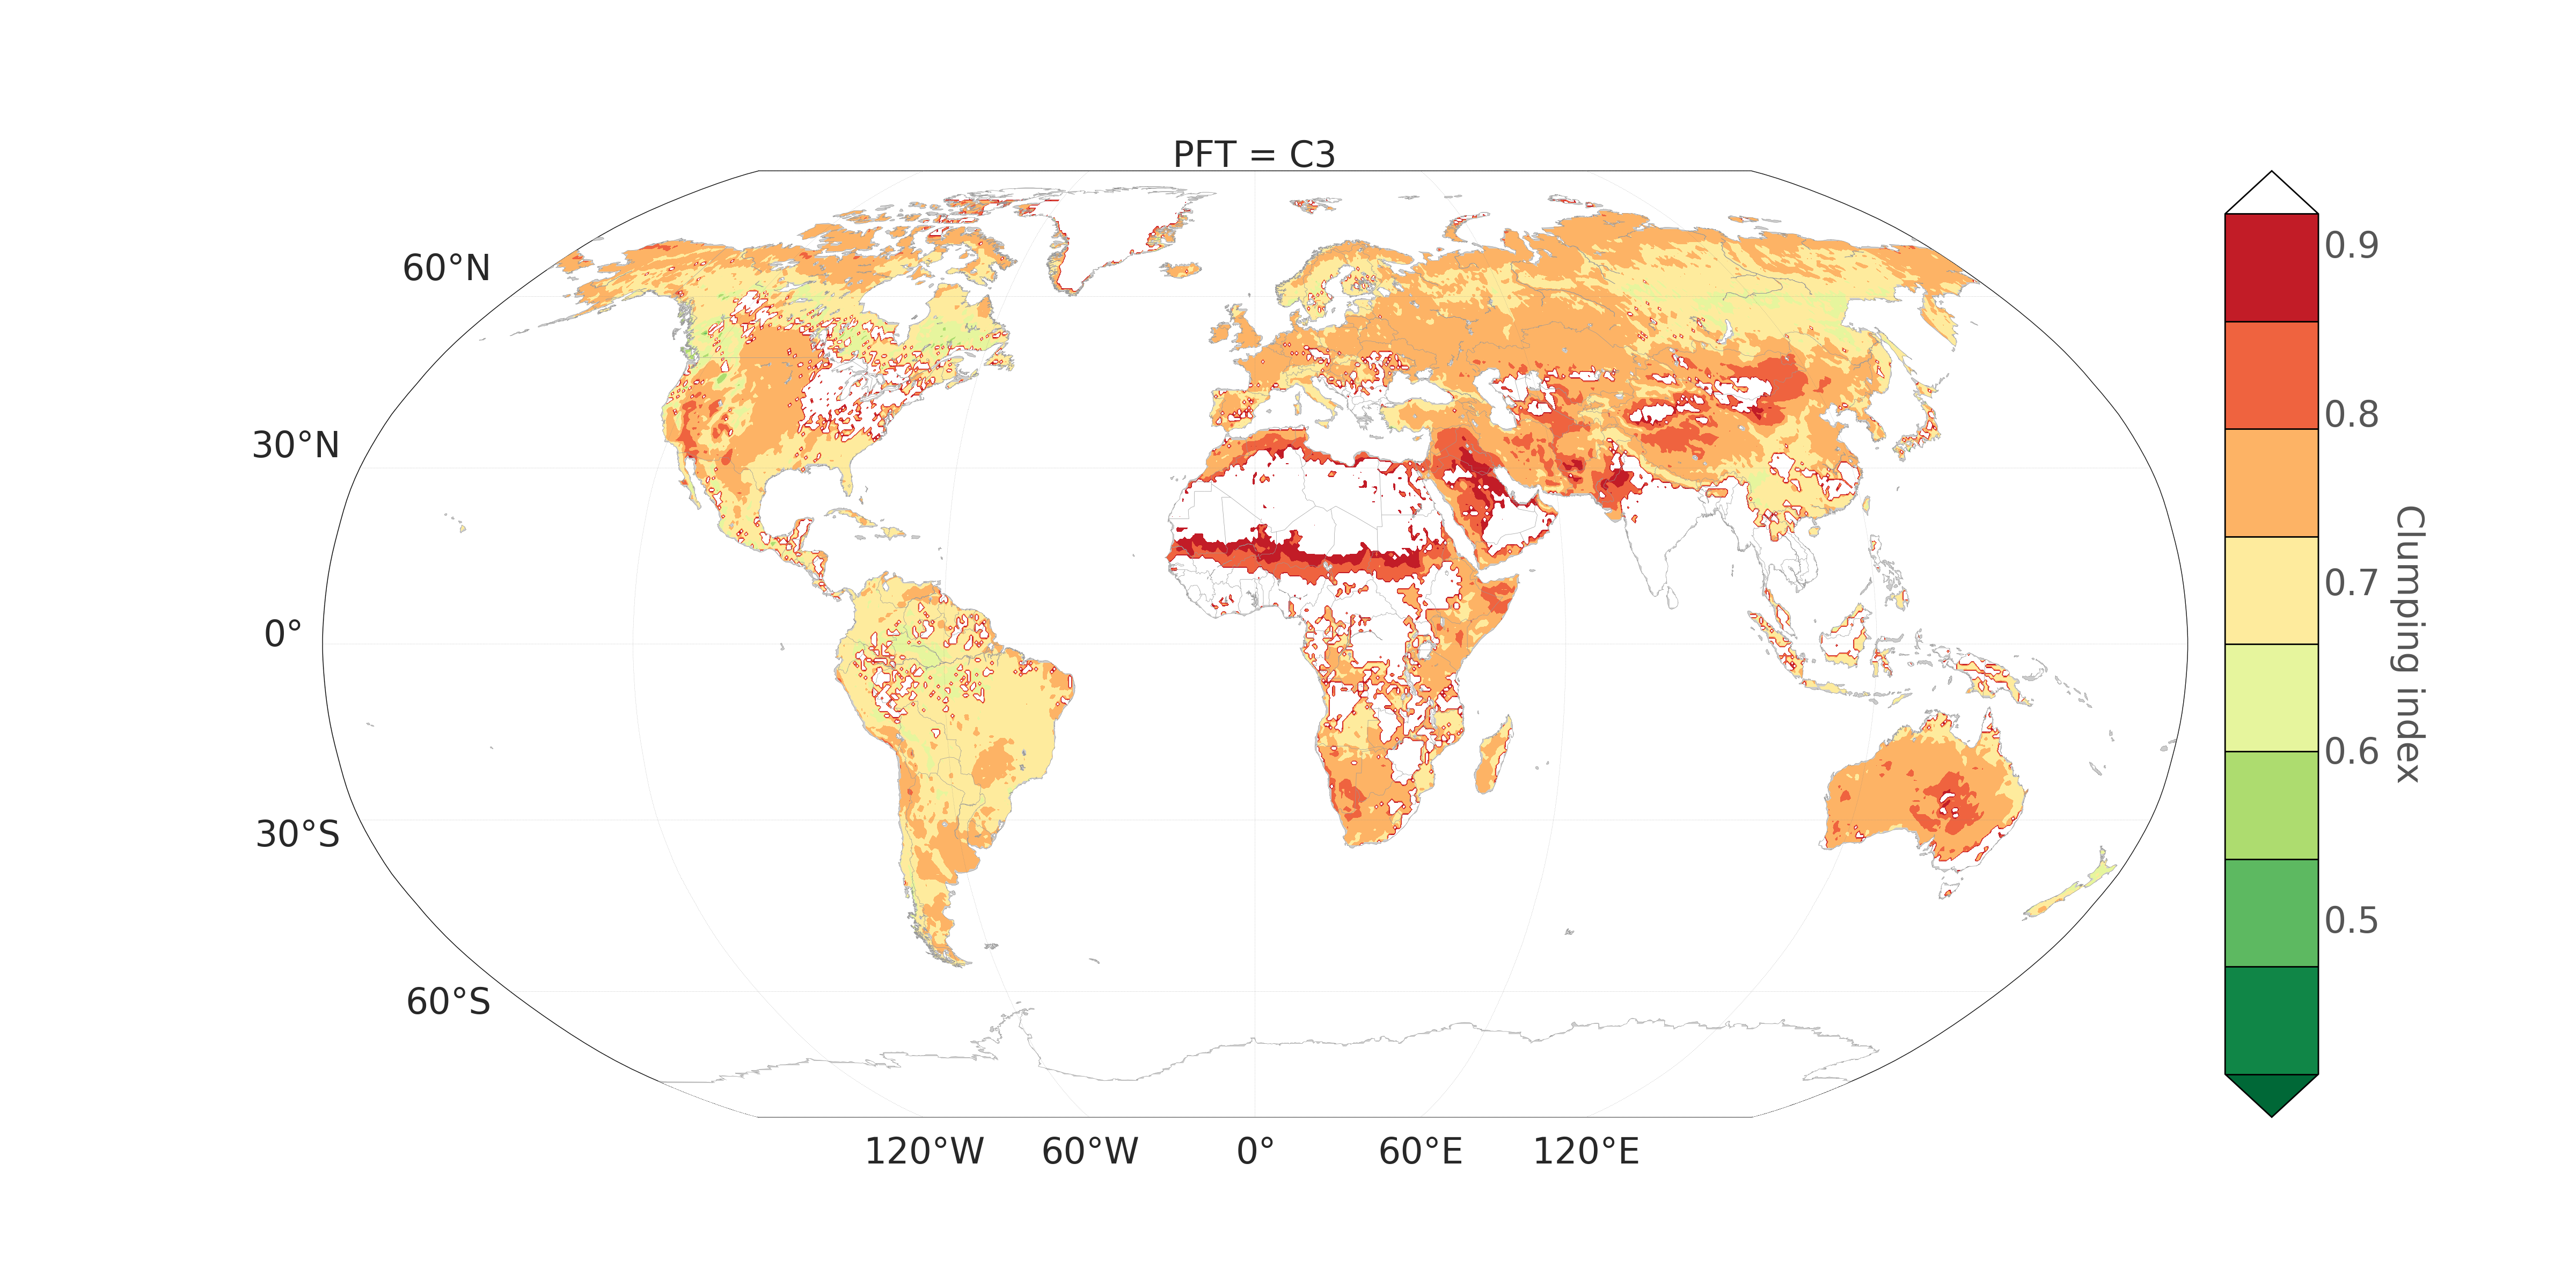
\includegraphics[width=0.5\textwidth]{/home/mn811042/Thesis/chapter6/figures_ofi/clump_PFT_2.png}}
\subfloat[C4]{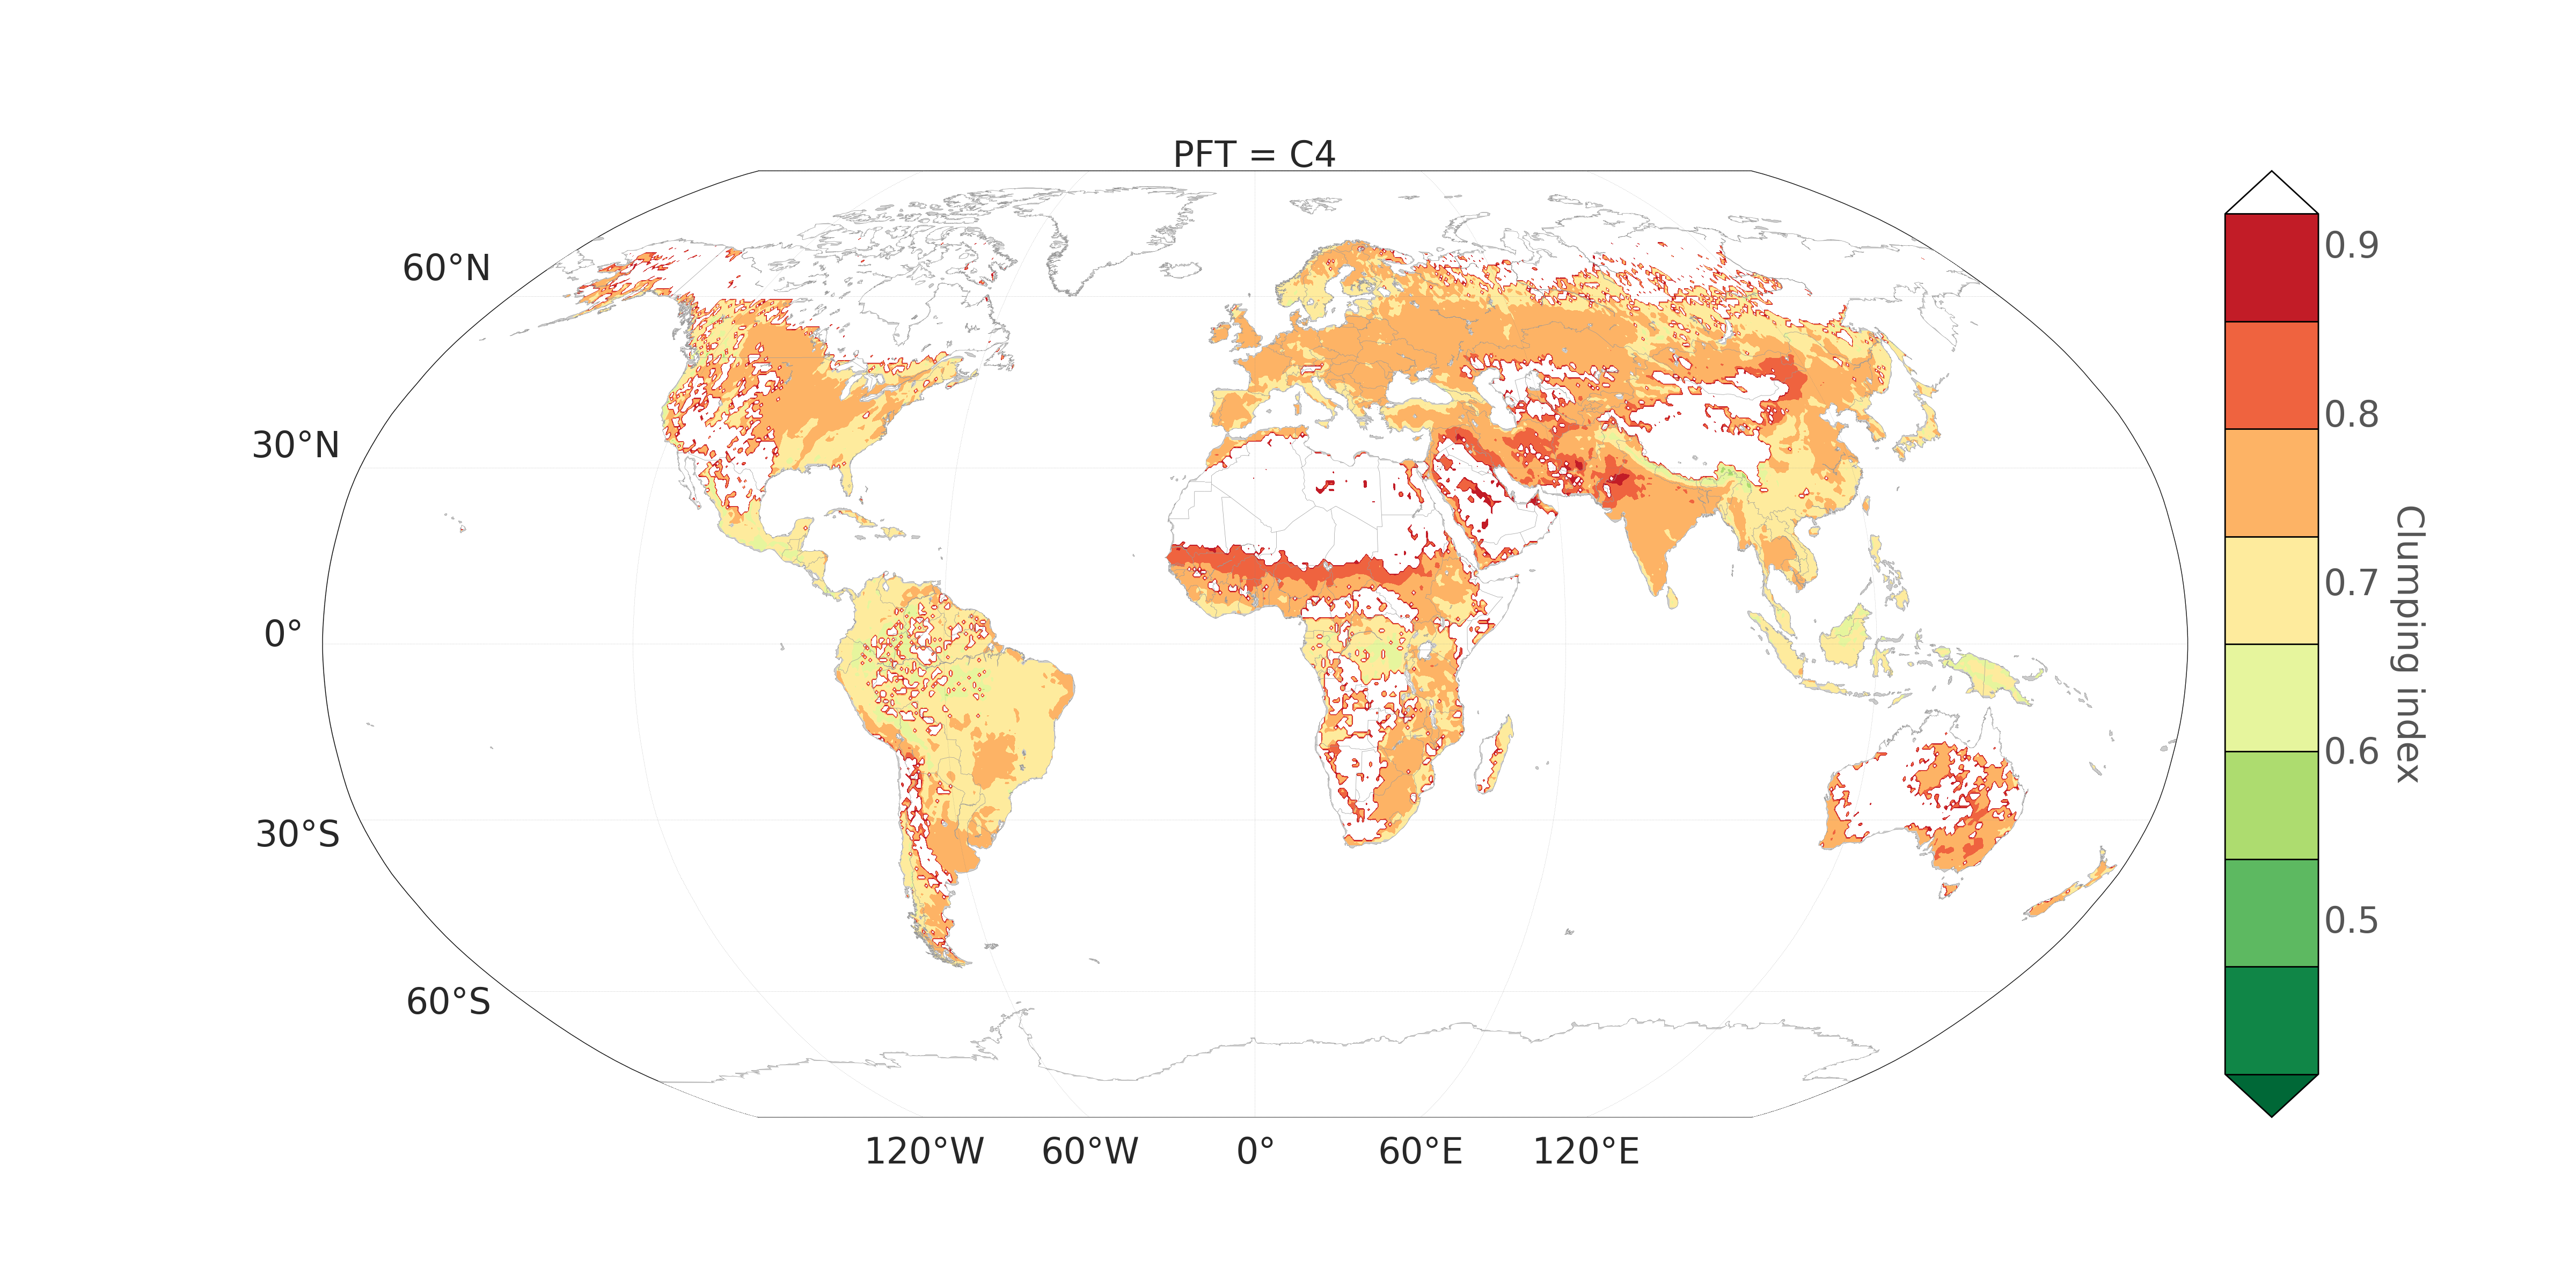
\includegraphics[width=0.5\textwidth]{/home/mn811042/Thesis/chapter6/figures_ofi/clump_PFT_3.png}}
\end{tabular}
\subfloat[SH]{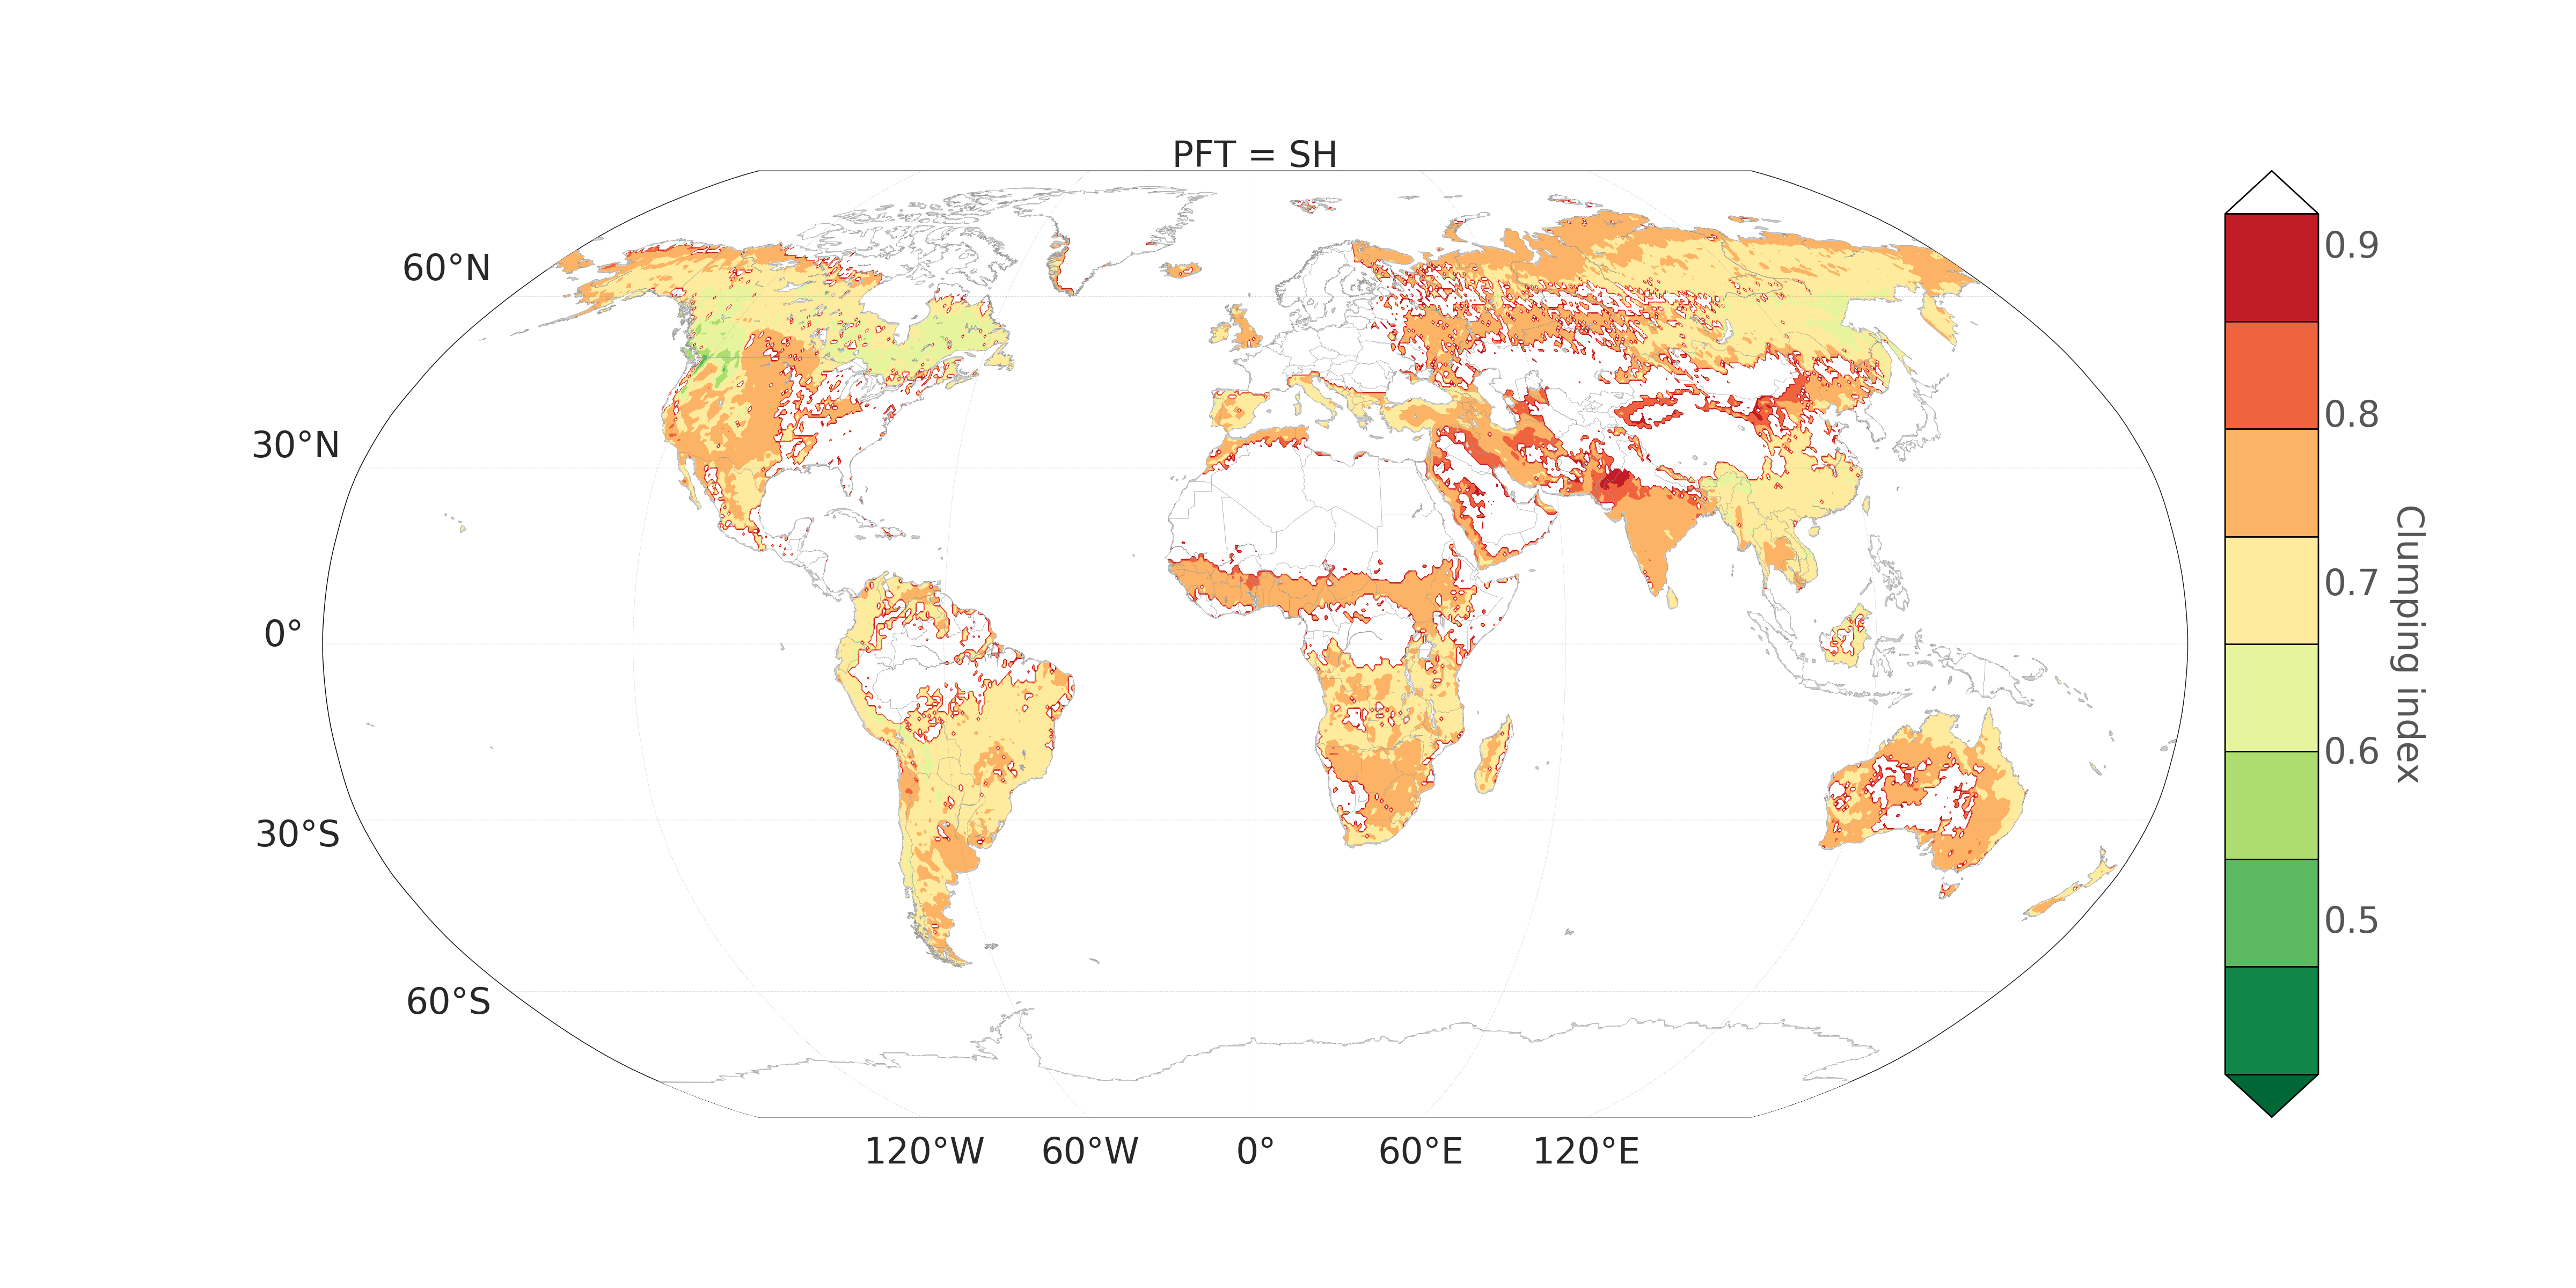
\includegraphics[width=0.5\textwidth]{/home/mn811042/Thesis/chapter6/figures_ofi/clump_PFT_4.png}}
\caption{Global map of MODIS-derived clumping index in 0.5$^{\circ}$ resolution for 2006 per PFT adapted from \citet{He2012} according to GLC-2000 land cover types.} 
\label{f:pgap}
\end{figure}


